\documentclass[12pt]{article}
\usepackage[utf8]{inputenc}

%allows you to neatly integrate an abstract once you start with the actual content
\usepackage{abstract}
\usepackage{microtype}
\usepackage{enumitem}

%%%%%%%%%%%%%%%%%%%%%%%%%%%%%%%%%%%%%%%%%%%%%%%%%%%%%%%%%%%%%%%%%%%%%%%%%%%%%%%%%%%%%%%%%% 
% SETTING THE GEOMETRY
%%%%%%%%%%%%%%%%%%%%%%%%%%%%%%%%%%%%%%%%%%%%%%%%%%%%%%%%%%%%%%%%%%%%%%%%%%%%%%%%%%%%%%%%%%

%borders and such
\usepackage
[
margin=1.5in
%a4paper,% other options: a3paper, a5paper, etc
%left=2.5cm,
%right=2.5cm, top=5cm,
% use vmargin=2cm to make vertical margins equal to 2cm.
% us  hmargin=3cm to make horizontal margins equal to 3cm.
% use margin=3cm to make all margins  equal to 3cm.
]
{geometry}
%makes for onehalfspacing in the whole document
\usepackage{setspace} 
\onehalfspacing
% \doublespacing
% allows to enter other margins for big figures or tables
\usepackage{changepage}
% disallow footnotes to extend over more than one page
\interfootnotelinepenalty=10000

%%%%%%%%%%%%%%%%%%%%%%%%%%%%%%%%%%%%%%%%%%%%%%%%%%%%%%%%%%%%%%%%%%%%%%%%%%%%%%%%%%%%%%%%%% 
% FONTS & COLORS
%%%%%%%%%%%%%%%%%%%%%%%%%%%%%%%%%%%%%%%%%%%%%%%%%%%%%%%%%%%%%%%%%%%%%%%%%%%%%%%%%%%%%%%%%% 
% Obviously colors. Usage: \color{red} Red text. This also allows you to make custom colors
\usepackage{xcolor}      
%if you want to start a multicolomns part inside your normally one columned article
\usepackage{multicol}
%titlesec allows you to change the way, titles are presented in latex
% \usepackage{titlesec}
%lets you change the style of your (sub)section headers
\usepackage{sectsty}
%I chose to make my headers cyan-colored
\sectionfont{\fontsize{16}{15}\selectfont}
\subsectionfont{\fontsize{14}{15}\selectfont}
\subsubsectionfont{\fontsize{12}{15}\selectfont}
% \subsectionfont{\color{cyan}}
% \subsubsectionfont{\color{cyan}}  
% \paragraphfont{\color{cyan}} 

% superscript 1st, 2nd, 3rd, 4th ... use \nth{8}
\usepackage[super]{nth}

%%%%%%%%%%%%%%%%%%%%%%%%%%%%%%%%%%%%%%%%%%%%%%%%%%%%%%%%%%%%%%%%%%%%%%%%%%%%%%%%%%%%%%%%%% 
% CITATION
%%%%%%%%%%%%%%%%%%%%%%%%%%%%%%%%%%%%%%%%%%%%%%%%%%%%%%%%%%%%%%%%%%%%%%%%%%%%%%%%%%%%%%%%%% 

\usepackage[english]{babel}
\usepackage{csquotes}

\usepackage[authordate,backend=biber,uniquename=false,uniquelist=false]{biblatex-chicago}
\bibliography{references}

\ExecuteBibliographyOptions{
    giveninits=true,
    % isbn=false,
    url=true,
    doi=true,
    % uniquename=init
    }
    
\DeclareBibliographyAlias{webpage}{online} 
\AtEveryBibitem{\clearlist{language}}
\AtEveryBibitem{%
      \ifentrytype{online}
        {}
        {\clearfield{urlyear}\clearfield{urlmonth}\clearfield{urlday}}
    }

%%%%%%%%%%%%%%%%%%%%%%%%%%%%%%%%%%%%%%%%%%%%%%%%%%%%%%%%%%%%%%%%%%%%%%%%%%%%%%%%%%%%%%%%%% 
% INSERTING PICTURES
%%%%%%%%%%%%%%%%%%%%%%%%%%%%%%%%%%%%%%%%%%%%%%%%%%%%%%%%%%%%%%%%%%%%%%%%%%%%%%%%%%%%%%%%%% 

%very useful if you want to add a jpfg or png file. Usage: \includegraphics{path/to/file}
\usepackage{grffile}
\usepackage{graphicx}
\usepackage{subcaption}
\usepackage[format=plain,
            % labelfont=it,
            font=footnotesize,
            % width=0.85\textwidth,
            % textfont=it,
            % singlelinecheck=on
            ]{caption}
% Figures can't live outside the section
\usepackage[section]{placeins}
% and then also \FloatBarrier at the end of a section to enforce harder.

% For figures turned 90 degrees
\usepackage{rotating}
% For uppercase subfigure panels
\renewcommand{\thesubfigure}{\Alph{subfigure}}


% Draw pictures, like game trees
\usepackage{tikz}
\usetikzlibrary{trees}
% Node styles
\tikzset{
% Two node styles for game trees: solid and hollow
solid node/.style={circle,draw,inner sep=1.5,fill=black},
hollow node/.style={circle,draw,inner sep=1.5,fill=white}
}
\usepackage{pgfplots}
\usepgfplotslibrary{fillbetween}


%%%%%%%%%%%%%%%%%%%%%%%%%%%%%%%%%%%%%%%%%%%%%%%%%%%%%%%%%%%%%%%%%%%%%%%%%%%%%%%%%%%%%%%%%% 
% INSERTING TABLES
%%%%%%%%%%%%%%%%%%%%%%%%%%%%%%%%%%%%%%%%%%%%%%%%%%%%%%%%%%%%%%%%%%%%%%%%%%%%%%%%%%%%%%%%%% 

\usepackage{array}
\usepackage{tabularx}
\usepackage{longtable}
\newcolumntype{x}[1]{>{\let\newline\\\arraybackslash\hspace{0pt}}p{#1}}
\newcolumntype{y}[1]{>{\centering\let\newline\\\arraybackslash\hspace{0pt}}p{#1}}
\newcolumntype{s}[1]{>{\centering\arraybackslash}p{#1}}
\renewcommand*{\arraystretch}{1.2}

\usepackage{multirow}

%%%%%%%%%%%%%%%%%%%%%%%%%%%%%%%%%%%%%%%%%%%%%%%%%%%%%%%%%%%%%%%%%%%%%%%%%%%%%%%%%%%%%%%%%% 
% LINKS AND WWW
%%%%%%%%%%%%%%%%%%%%%%%%%%%%%%%%%%%%%%%%%%%%%%%%%%%%%%%%%%%%%%%%%%%%%%%%%%%%%%%%%%%%%%%%%% 

% Provides clickable links in the PDF-document for \ref and the TOC
\usepackage[]{hyperref} %you can remove the hidelinks option to make the hyperrefs visible. looks very ugly to me, but might be useful to less experienced readers of pdfs
% Lets you typeset urls with linebreak. Usage: \url{http://...}  
\usepackage{url}

%%%%%%%%%%%%%%%%%%%%%%%%%%%%%%%%%%%%%%%%%%%%%%%%%%%%%%%%%%%%%%%%%%%%%%%%%%%%%%%%%%%%%%%%%% 
% CODE INTEGRATION
%%%%%%%%%%%%%%%%%%%%%%%%%%%%%%%%%%%%%%%%%%%%%%%%%%%%%%%%%%%%%%%%%%%%%%%%%%%%%%%%%%%%%%%%%% 

% Source Code Listings. Usage: \begin{lstlisting}...\end{lstlisting}
\usepackage{listings}
%this defines a lot of parameters for code. makes it look nice IMO
\lstset{ 
	breaklines=true,                 % sets automatic line breaking
	commentstyle=\color{mygreen},    % comment style
	escapeinside={\%*}{*)},          % if you want to add LaTeX within your code
	frame=single,	                   % adds a frame around the code
	keepspaces=true,                 % keeps spaces in text, useful for keeping indentation of code (possibly needs columns=flexible)
	keywordstyle=\color{blue},       % keyword style
	numbers=left,                    % where to put the line-numbers; possible values are (none, left, right)
	numbersep=5pt,                   % how far the line-numbers are from the code
	numberstyle=\tiny\color{mygray}, % the style that is used for the line-numbers
	rulecolor=\color{black},         % if not set, the frame-color may be changed on line-breaks within not-black text (e.g. comments (green here))
	showspaces=false,                % show spaces everywhere adding particular underscores; it overrides 'showstringspaces'
	showstringspaces=false,          % underline spaces within strings only
	showtabs=false,                  % show tabs within strings adding particular underscores
	stepnumber=2,                    % the step between two line-numbers. If it's 1, each line will be numbered
	stringstyle=\color{mymauve},     % string literal style
	tabsize=2,	                   % sets default tabsize to 2 spaces
	title=\lstname                   % show the filename of files included with \lstinputlisting; also try caption instead of title
}         

%%%%%%%%%%%%%%%%%%%%%%%%%%%%%%%%%%%%%%%%%%%%%%%%%%%%%%%%%%%%%%%%%%%%%%%%%%%%%%%%%%%%%%%%%% 
% MATH
%%%%%%%%%%%%%%%%%%%%%%%%%%%%%%%%%%%%%%%%%%%%%%%%%%%%%%%%%%%%%%%%%%%%%%%%%%%%%%%%%%%%%%%%%% 

%some very useful packages for writing down beautiful formulas
\usepackage{amsmath}
\usepackage{amssymb}
\usepackage{mathtools}
\usepackage{mathrsfs}  
\usepackage{bm}
\usepackage{empheq}
% Nice rules for tables. Usage \begin{tabular}\toprule ... \midrule ... \bottomrule
\usepackage{booktabs}          

%%%%%%%%%%%%%%%%%%%%%%%%%%%%%%%%%%%%%%%%%%%%%%%%%%%%%%%%%%%%%%%%%%%%%%%%%%%%%%%%%%%%%%%%%% 
% APPENDIX
%%%%%%%%%%%%%%%%%%%%%%%%%%%%%%%%%%%%%%%%%%%%%%%%%%%%%%%%%%%%%%%%%%%%%%%%%%%%%%%%%%%%%%%%%% 

\usepackage{appendix}
% Change numbering of figures, tabels etc. in Appendix
\usepackage{chngcntr} 

\usepackage{titletoc}


%%%%%%%%%%%%%%%%%%%%%%%%%%%%%%%%%%%%%%%%%%%%%%%%%%%%%%%%%%%%%%%%%%%%%%%%%%%%%%%%%%%%%%%%%% 
% ALL ABOUT YOU
%%%%%%%%%%%%%%%%%%%%%%%%%%%%%%%%%%%%%%%%%%%%%%%%%%%%%%%%%%%%%%%%%%%%%%%%%%%%%%%%%%%%%%%%%% 


\title{22BDP Macroeconomics week 4}
\author{Tom Rodriguez, Bénédicte Droz}
\date{06.08.2023}

%start your document with \begin{document} and type everything inbetween \begin{document} and \end{document}
\begin{document}

\begin{titlepage}
	
	\newcommand{\HRule}{\rule{\linewidth}{0.5mm}} % Defines a new command for the horizontal lines, change thickness here
	
	\center % Center everything on the page
	
	%----------------------------------------------------------------------------------------
	%	HEADING SECTIONS
	%----------------------------------------------------------------------------------------
	
% 	\includegraphics{Figures/UZH.eps} \\[1.5cm] 
    %	\textsc{\LARGE University of Zurich}\\[1.5cm] % Name of your university/college and the size of the distance to the next line. \LARGE is used to make really big fonts
	\textsc{\large Beginning Doctoral Program Gerzensee}\\[0.5cm] % Major heading such as course name
	{\large Lectures held by Ricardo Reis and Fernando Alvarez}\\[1cm] % you can the name(s) of your instructor(s)
	
	
	%----------------------------------------------------------------------------------------
	%	TITLE SECTION
	%----------------------------------------------------------------------------------------
	
	\HRule \\[1.0cm]
	{ \LARGE \bfseries Macroeconomics Midterm Solutions}\\[0.4cm] % Title of your document, and yes, I am aware that it is stupid to have to list it twice. I don't know how to work around this.
	\HRule \\[2cm]
	
	%----------------------------------------------------------------------------------------
	%	AUTHOR SECTION
	%----------------------------------------------------------------------------------------
	

	
	\begin{flushleft}
        \Large List of Contributors:
        
		{\large 
            \href{https://rodrigueztom.github.io}{Tom Rodriguez (University of Fribourg)}
        }
	\end{flushleft}
	
	
	%----------------------------------------------------------------------------------------
	%	DATE SECTION
	%----------------------------------------------------------------------------------------
	
	{\large \today} % Date, change the \today to a set date if you want to be precise
	
	% Fill the rest of the page with whitespace
	\vfill 
	
\end{titlepage}

%%%%%%%%%%%%%%%%%%%%%%%%%%%%%%%%%%%%%%%%%%%%%%%%%%%%%%%%%%%%%%%%%%%%%%%%%%%%%%%%%%%%%%%%%% 
% GEOMETRY according to university guidelines
%%%%%%%%%%%%%%%%%%%%%%%%%%%%%%%%%%%%%%%%%%%%%%%%%%%%%%%%%%%%%%%%%%%%%%%%%%%%%%%%%%%%%%%%%% 

%This line can be used to adjust the geometry of the document according to the university guidelines for borders and such
% \newgeometry{margin=1.5in}

%%%%%%%%%%%%%%%%%%%%%%%%%%%%%%%%%%%%%%%%%%%%%%%%%%%%%%%%%%%%%%%%%%%%%%%%%%%%%%%%%%%%%%%%%% 
% ABSTRACT
%%%%%%%%%%%%%%%%%%%%%%%%%%%%%%%%%%%%%%%%%%%%%%%%%%%%%%%%%%%%%%%%%%%%%%%%%%%%%%%%%%%%%%%%%% 

%\thispagestyle{empty} %suppresses the footer and header since I want to start show them after the TOC, optional
\pagenumbering{roman}	
% \tableofcontents

% The \clearpage command is a pagebreak to separate the abstract from the content
%\clearpage
\newpage
\pagenumbering{arabic}

%%%%%%%%%%%%%%%%%%%%%%%%%%%%%%%%%%%%%%%%%%%%%%%%%%%%%%%%%%%%%%%%%%%%%%%%%%%%%%%%%%%%%%%%%% 
 % ACTUAL CONTENT 
%%%%%%%%%%%%%%%%%%%%%%%%%%%%%%%%%%%%%%%%%%%%%%%%%%%%%%%%%%%%%%%%%%%%%%%%%%%%%%%%%%%%%%%%%%

\newpage
\section{Microeconomics Midterm 2014 / 15}

{
\subsection*{Schmidt}

\subsubsection*{Exercise 1}

\begin{enumerate}[label=(\alph*)]
{\item 
\begin{align*}
    x_{1}(\lambda p, \lambda w)=\lambda^{1+\alpha-\delta} \frac{p_{1}^{\alpha} w}{p_{1}^{\delta}+p_{2}^{\delta}+p_{3}^{\delta}}=\lambda^{1+\alpha-\delta} x_{1}(p, w)
\end{align*}

Must have $1+\alpha-\delta=0$ or $\alpha=\delta-1$

\begin{align*}
    x_{2}(\lambda p, \lambda w)=\lambda^{1+\alpha-\delta} \frac{p_{2}^{\alpha} w}{p_{1}^{\delta}+p_{2}^{\delta}+p_{3}^{\delta}}+\beta \frac{p_{1}}{p_{3}} \frac{\lambda}{\lambda}
\end{align*}

No restriction on $\beta$.

\begin{align*}
    x_{3}(\lambda p, \lambda w)=\lambda^{1+\alpha-\sigma} \frac{\gamma p_{3}^{\alpha} w}{p_{1}^{\delta}+p_{2}^{\delta}+p_{3}^{\delta}}=\lambda^{1+\alpha-\delta} x_{3}(p, w)
\end{align*}

No restriction on $\gamma$.

In summary, we only need $\alpha=\delta-1$.
}
{\item 

\begin{align*}
    p_{1} x_{1}(\cdot)+p_{2} x_{2}(\cdot)+p_{3} x_{3}(\cdot) &= w \quad \text{to satisfy Walras' Law} \\
    \Leftrightarrow \frac{w}{p_{1}^{\delta}+p_{2}^{\sigma}+p_{3}^{\sigma}}\left[p_{1}^{1+\alpha}+p_{2}^{1+\alpha}+\gamma p_{3}^{1+\alpha}\right]+\beta \frac{p_{1} p_{2}}{p_{3}} &= w
\end{align*}

Must have $\beta=0$ :

\begin{align*}
    p_{1}^{\delta}+p_{2}^{\delta}+p_{3}^{\delta}=p_{1}^{1+\alpha}+p_{2}^{1+\alpha}+\gamma p_{3}^{1+\alpha}
\end{align*}

Must have $\gamma=1$ \& $\alpha=\delta-1$.

In summary:

\begin{align*}
    \alpha=\delta-1 \quad \beta=0 \quad \gamma=1
\end{align*}
}
\end{enumerate}
}
{
\subsubsection*{Exercise 2}

\begin{enumerate}[label=(\alph*)]
{\item 
Invert $e(p,u)$ as in equilibrium: $e(p, u)=w$ and also $u=v(p, w)$

\begin{align*}
    v\left(p, w\right)=w \frac{p_{1}+p_{2}}{p_{1} p_{2}}=w\left[\frac{1}{p_{1}}+\frac{1}{p_{2}}\right]
\end{align*}
}
{\item 
Roy's Identity

\begin{align*}
    x_1\left(p_1 w\right)=-\frac{\frac{\partial v(\cdot)}{\partial p_1}}{\frac{\partial v(\cdot)}{\partial w}}=\frac{w \frac{1}{p_1^2}}{\frac{p_1+p_2}{p_1 p_2}}=\frac{w}{p_1+p_2}\frac{p_2}{p_1} \\
    x_2\left(p_1 w\right)=\frac{w}{p_1+p_2} \frac{p_1}{p_2} \text { by symmetry }
\end{align*}
}
{\item 
\begin{align*}
    & \frac{x_1\left(p, w\right)}{x_2\left(p, w\right)}=\left(\frac{p_1}{p_2}\right)^{-2} \\
    & \eta_{12}=-(-2)\left(\frac{p_1}{p_2}\right)^{-3} \frac{\frac{p_1}{p_2}}{\left(\frac{p_1}{p_2}\right)^{-2}}=2
\end{align*}
}
\end{enumerate}
}
{
\subsubsection*{Exercise 2}

\begin{enumerate}[label=(\alph*)]
{\item 
Invert $e(p,u)$ as in equilibrium: $e(p, u)=w$ and also $u=v(p, w)$

\begin{align*}
    v\left(p, w\right)=w \frac{p_{1}+p_{2}}{p_{1} p_{2}}=w\left[\frac{1}{p_{1}}+\frac{1}{p_{2}}\right]
\end{align*}
}
{\item 
Roy's Identity

\begin{align*}
    x_1\left(p_1 w\right)=-\frac{\frac{\partial v(\cdot)}{\partial p_1}}{\frac{\partial v(\cdot)}{\partial w}}=\frac{w \frac{1}{p_1^2}}{\frac{p_1+p_2}{p_1 p_2}}=\frac{w}{p_1+p_2}\frac{p_2}{p_1} \\
    x_2\left(p_1 w\right)=\frac{w}{p_1+p_2} \frac{p_1}{p_2} \text { by symmetry }
\end{align*}
}
{\item 
CES utility:

\begin{align*}
    u\left(x_1, x_2\right)=\left[\frac{1}{2} x_1^\rho+\frac{1}{2} x_2^\rho\right]^{\frac{1}{\rho}} \text { where } \rho=1-\frac{1}{n_{12}}=1 / 2
\end{align*}
}
\end{enumerate}
}
{
\subsubsection*{Exercise 3}

The difference between consumer theory and production theory is mainly the fact that firms do not have budget constraints.
This problem introduces a budget constraint. Therefore, we are going to treat the problem like a consumer problem.
In that sense, the revenue is comparable to the utility function, and the cash constraint is like the wealth of a consumer.
Consequently, we are solving the following revenue maximization problem (which is the analogue to a utility maximization problem):

\begin{align*}
    \max_{z_1,z_2} pf(z_1,z_2) \\
    \operatorname{s.t.} \; w_1z_1 + w_2z_2 \leq C
\end{align*}

We will assume an interior solution (the budget constraint is binding).
Then, the revenue function $R(p, w_1, w_2, C)$ that the exercise gives us is just the equivalent to the indirect utility.

\begin{enumerate}[label=(\alph*)]
{\item 
As $R(p, w_1, w_2, C)$ works like the indirect utility, we apply Roy's identity to find the factor demand, which is the analogue to the Walrasian demand:

\begin{align*}
    z_1&=-\frac{\frac{\partial R}{\partial w_1}}{\frac{\partial R}{\partial C}} \\
    &= -\frac{p \cdot(-\alpha) \frac{1}{w_1}}{p \cdot \frac{1}{C}} \\
    &= \alpha \frac{C}{w_1}
\end{align*}
}
{\item 
We treat $R(p,w,C)$ as the indirect utility depending on income and invert it to find the cost function $C(p,w,R)$, which is the analogue to the expenditure function in consumer theory:

\begin{align*}
    R&=p\left[\gamma+\ln C(p,w,R)-\alpha \ln w_1-(1-\alpha) \ln w_2\right] \\
    \frac{R}{p}-\gamma &= \ln \left(\frac{C(p,w,R)}{w_1^\alpha w_2^{1-\alpha}} \right) \\
    \exp\left(\frac{R}{p}-\gamma\right)&=\frac{C(p,w,R)}{w_1^\alpha w_2^{1-\alpha}} \\
    C(p,w,R) &= w_1^\alpha w_2^{1-\alpha}\exp\left(\frac{R}{p}-\gamma\right)
\end{align*}
}
{\item 
Since the cost function from (b) happens to be the analogue to the expenditure function, we can apply Shephard's Lemma in order to find the factor demand for a given $R$ at minimum cost, as this is the analogue to the Hicksian demand in consumer theory.
In that spirit, let us call this function $h_1(p,w,R)$.

\begin{align*}
    h_1(p,w,R)&=\frac{\partial C\left(w,R\right)}{\partial w_1} \\
    &= \alpha \exp \left[\frac{R}{p}-\gamma\right] \cdot\left(\frac{w_2}{w_1}\right)^{1-\alpha}
\end{align*}
}
{\item 
In consumer theory, the Hicksian demand and the Walrasian demand meet at optimum. We can also show that here:

\begin{align*}
    h_1(w,R)&=z_1^* \\
    \alpha \exp \left[\frac{R}{p}-\gamma\right] \cdot\left(\frac{w_2}{w_1}\right)^{1-\alpha}&=\alpha \frac{C}{w_1}\\
    \exp \left[\frac{R}{p}-\gamma\right] w_1^\alpha w_2^{1-\alpha}&=C \\
    \frac{R}{p}-\gamma &= \ln \left(\frac{C}{w_1^\alpha w_2^{1-\alpha}} \right) \\
    R&=p\left[\gamma+\ln C-\alpha \ln w_1-(1-\alpha) \ln w_2\right]
\end{align*}

The last line is exactly the formula for the revenue that is observed by our econometrician friend in the optimum. Therefore, we have shown that the two demands are equal whenever the firm is acting optimally, i.e. maximizing its revenue or minimizing its cost. Put differently, the revenue maximization problem is the dual problem to the cost minimization problem and vice versa.
}
\end{enumerate}
}

\newpage
{
\subsection*{Gottardi}

\subsubsection*{Exercise 1}

\begin{enumerate}[label=(\alph*)]
{\item 
True. We need three things for FWT:

\begin{itemize}
    \item LNS, which is satisfied by monotonicity
    \item Complete markets, satisfied by two prices for two commodities
    \item free disposal (given)
\end{itemize}
}
{\item 
False. Convexity is violated by B. Consider the following illustration:

\begin{figure}[!ht]
    \centering
    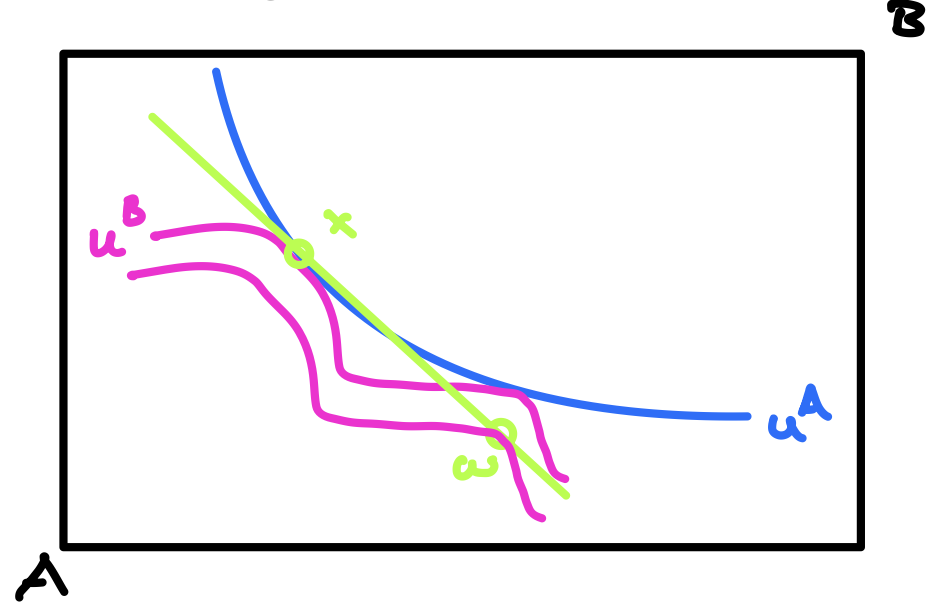
\includegraphics[width=0.75\linewidth]{images/2014_15_1.png}    
\end{figure}

Because $B$ has non-convex preferences, $x$ is not a CE. Actually no CE exists.
}
{\item 
False by same argument as in (b).
}
\end{enumerate}
}
{
\subsubsection*{Exercise 2}

\begin{enumerate}[label=(\alph*)]
{\item 
PE allocations are along $x_{1}^{A}=x_{2}^{A}$. If we are at any other point, just give some to $B$ because $A$ only cares about lower amount.

\begin{figure}[!ht]
    \centering
    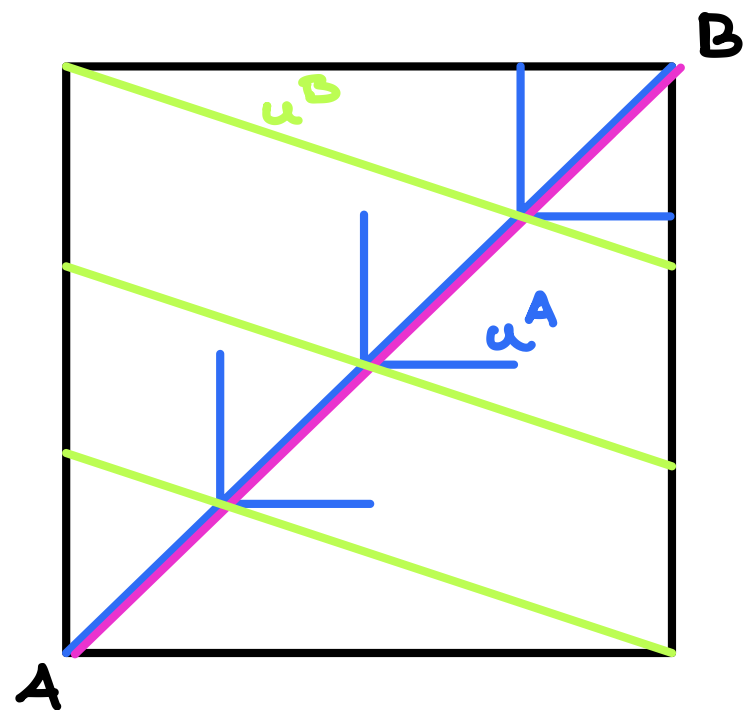
\includegraphics[width=0.75\linewidth]{images/2014_15_2.png}    
\end{figure}
}
{\item 
Let $p=\frac{p_{1}}{p_{2}}$

\underline{Consumer A:}

\begin{align*}
    x_{1}^{A}=x_{2}^{A} \quad\text{BC: } p x_{1}^{A}+x_{2}^{A}=6 p+2
\end{align*}

\underline{Consumer B:}

\begin{align*}
    x_1^B=\left\{\begin{array}{lll}
        \infty & \text { if } & p<1 / 3 \\
        \mathbb{R}^{+} & \text {if } & p=1 / 3 \\
        0 & \text { if } & \rho>1 / 3
    \end{array}\right. 
    \quad ; \quad
    x_2^B=\left\{\begin{array}{lll}
        \infty & \text { if } & p>1 / 3 \\
        \mathbb{R}^{+} & \text {if } & p=1 / 3 \\
        0 & \text { if } & p<1 / 3
    \end{array}\right. \\
    \text{BC: } p x_1^B+x_2^B=2 p+6
\end{align*}

\underline{Market Clearing:}

\begin{align*}
    & x_1^A+x_1^B = w_1^A+w_1^B=8 \\
    & x_2^A+x_2^B = w_2^A+w_2^B=8
\end{align*}

use $x_1^A=x_2^A \longrightarrow x_1^B=x_2^B$. Therefore $p=\frac{1}{3}$ so no excess demand for either good.

By $\operatorname{BC}^A$:

\begin{align*}
    & x_1^A=x_2^A=3 \\
    & x_1^B=x_2^B=5
\end{align*}

\underline{Competitive Equilibrium:}

\begin{align*}
    \left(x_1^A, x_2^A\right) & =(3,3) \\
    \left(x_1^B, x_2^B\right) & =(5,5) \\
    p & =\frac{1}{3}
\end{align*}

This is PE since $x_1^A = x_2^A$.
}
{\item 
Yes. The reason is that $p=\frac{1}{3}$ is the only possible equilibrium price. Otherwise markets cannot clear \& we have excess demand for one of the commodities.
}
\end{enumerate}
}
{
\subsubsection*{Exercise 3}

$w^1=(8,4) \text {; } \quad w^2=(2,6)$

\begin{enumerate}[label=(\alph*)]
{\item 
Note that we have (1) identical beliefs
and (2) no aggregate risk as $w_{1}=w_{2}=10$.

Therefore, full risk sharing is possible and $x_{1}^{h}=x_{2}^{h} \quad \forall h$ is PE. I.e. the $45^{\circ}$-line:

\begin{figure}[!ht]
    \centering
    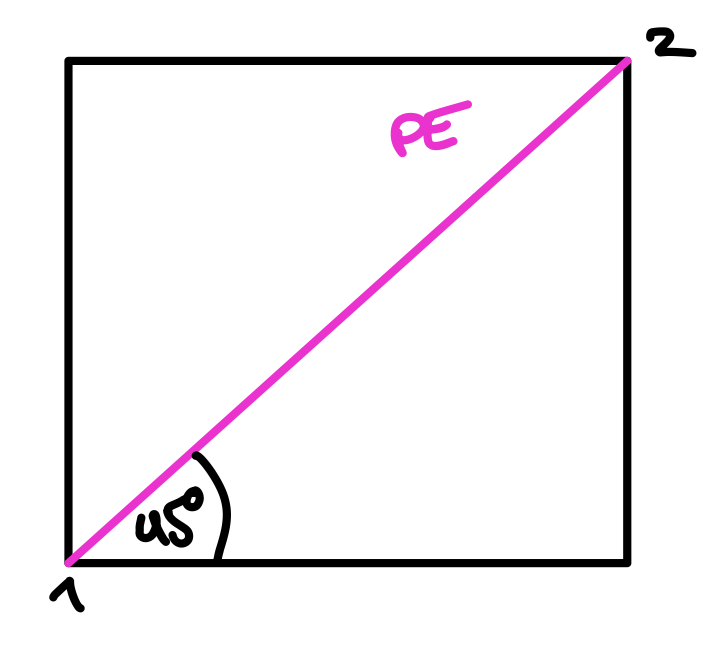
\includegraphics[width=.75\textwidth]{images/2014_15_3.png}
\end{figure}
}
{\item 
\underline{Consumer h:}

\begin{align*}
    \max_{x_{1}^{h}, x_{2}^{h}} \quad & \pi u^{h}\left(x_{1}^{h}\right)+(1-\pi) u^{h}\left(x_{2}^{h}\right) \\
    \text { s.t. } \quad & q_{1} \theta_{1}^{h}+q_{2} \theta_{2}^{h}=0 \\
    & x_{1}^{n}=w_{1}^{h}+\theta_{1}^{h} \\
    & x_{2}^{u}=w_{1}^{h}+\theta_{2}^{h}
\end{align*}

Plug in the $\theta$s:

\begin{align*}
    \max _{x_{1}^{h}, x_{2}^{h}} \quad & \pi u^{h}\left(x_{1}^{h}\right)+(1-\pi) u^{h}\left(x_{2}^{h}\right) \\
    \text { s.t. } & q_{1}\left(x_{1}^{h}-w_{1}^{h}\right)+q_{2}\left(x_{2}^{h}-w_{2}^{h}\right)=0
\end{align*}

FOCs:

\begin{align*}
    \pi \frac{\partial u^{h}\left(x_{1}^{h}\right)}{\partial x_{1}^{h}}-\lambda q_{1}&=0 \\
    (1-\pi) \frac{\partial u^{h}\left(x_{2}^{h}\right)}{\partial x_{2}^{h}}-\lambda q_{2} &= 0 \\
    \Longrightarrow \quad \frac{q_{1}}{q_{2}} &= \frac{\pi}{1-\pi} \frac{\frac{\partial u^{h}\left(x_{1}^{h}\right)}{\partial x_{1}^{h}}}{\frac{\partial u^{h}\left(x_{2}^{h}\right)}{\partial x_{2}^{h}}}
\end{align*}

Perfect risk sharing implies: $x_{1}^{h} = x_{2}^{h}$, and therefore we have 

\begin{align*}
    \frac{q_1}{q_2}=\frac{\pi}{1-\pi}
\end{align*}

Plug this into the BC:

\begin{align*}
    \frac{q_{1}}{q_{2}}\left(x_{1}^{h}-w_{1}^{h}\right)+x_{1}^{h}-w_{2}^{h} &= 0 \\
    x_{1}^{h}\left(\frac{q_{1}}{q_{2}}+1\right) &= w_{2}^{h}+w_{1}^{h} \frac{q_{1}}{q_{2}} \\
    x_{1}^{h}=x_{2}^{h}=\left(\frac{q_{1}}{q_{2}}+1\right)^{-1}\left(w_{2}^{h}+w_{1}^{h} \frac{q_{1}}{q_{2}}\right) 
    &= (1-\pi)\left(w_{2}^{h}+w_{1}^{h} \frac{\pi}{1-\pi}\right) 
    =\pi w_{1}^{h}+(1-\pi) w_{2}^{h} \\
    x_{1}^1=x_{2}^1 &= \pi 8+(1-\pi) 4=4(1+\pi) \\
    x_{1}^{2}=x_{2}^{2} &= \pi 2+(1-\pi) 6=6-4 \pi
\end{align*}

\underline{Competitive Equilibrium: }

\begin{align*}
    \left(x_1^1, x_2^1\right) & =(4+4 \pi, 4+4 \pi) \\
    \left(x_1^2, x_2^2\right) & =(6-4 \pi, 6-4 \pi) \\
    \frac{q_1}{q_2} & =\frac{\pi}{1-\pi}
\end{align*}
}
\end{enumerate}
}\newpage
\section{Microeconomics Midterm 2015 / 16}

{
\subsection*{Schmidt}

\subsubsection*{Exercise 1}

\begin{enumerate}[label=(\alph*)]
{\item 
To violate WARP:

find $w$ by Walras law

$$
\begin{aligned}
& \left|\begin{array}{l}
p^{\prime} y \leqslant w^{\prime} \\
p y^{\prime} \leqslant w
\end{array}\right| \\
\Leftrightarrow&\left|\begin{array}{l}
30(12+x) \leqslant 600 \\
10(30+24) \leqslant 360+24 x
\end{array}\right| \\
\Leftrightarrow& \left|\begin{array}{l}
30 x \leqslant 240 \\
180 \leqslant 24 x
\end{array}\right| \\
\Leftrightarrow& \left|\begin{array}{l}
30 x \leqslant 240 \\
180 \leqslant 24 x
\end{array}\right| \\
\Leftrightarrow& \left|\begin{array}{c}
x \leqslant 8 \\
7.5 \leqslant x
\end{array}\right|
\end{aligned}
$$

WARP is violated for $x \in[7.5,8]$.
}
{\item
Bundle 2 must be affordable in period 1. Then we see that the consumer chooses bundle 1 over bundle 2: $x \leqslant 8$ by (a)

To not violate WARP we find that if and only if $x \in[0,7.5)$, bundle 1 is revealed preferred.
}
{\item 
The quantity increased. To have an inferior good, $\frac{\partial y_{1}}{\partial w}<0$. Thus, income must have decreased:

$$
\begin{aligned}
600 & \leqslant 360+24 x \\
\Leftrightarrow 10 & \leqslant x
\end{aligned}
$$

We find that good 1 is inferior for $x \geqslant 10$.
}
\end{enumerate}
}
{
\subsubsection*{Exercise 2}

Monotone transformation to $u_{2}(\cdot)$ :

$$
\tilde{u}_{2}\left(x_{1}, x_{2}\right)=x_{1}^{\frac{3}{3+a}} x_{2}^{\frac{a}{3+a}}
$$

\begin{enumerate}[label=(\alph*)]
{\item
consumer 1: Invert $e_{1}(\cdot)$. In equilibrium $e_{1}(\cdot)=w_{1}$ and $v_{1}\left(p, w_{1}\right)=u_{1}$ :

$$
\begin{aligned}
& w_{1}=v_{1}\left(p, w_{1}\right) \sqrt{p_{1} p_{2}} \\
\Leftrightarrow \quad & v_{1}\left(p, w_{1}\right)=\frac{w_{1}}{\sqrt{p_{1} p_{2}}}
\end{aligned}
$$

Apply Roy's identity:

$$
x_{1}^{1}\left(p_{1}, w_{1}\right)=-\frac{\frac{\partial v_{1}(\cdot)}{\partial p_{1}}}{\frac{\partial v_{1}(\cdot)}{\partial w}}=-\frac{-\frac{1}{2} p_{1}^{-3/2} \frac{w}{\sqrt{p_{2}}}}{\frac{1}{\sqrt{p_{1} p_{2}}}}
$$

$$
x_{1}^{1}\left(p_{1}, w_{1}\right)=\frac{1}{2} \frac{w_{1}}{p_{1}}
$$

By symmetry of $v_{1}\left(p, w_{1}\right)$ :

$$
x_{2}^{1}\left(p_{1}, w_{1}\right)=\frac{1}{2} \frac{w_{1}}{p_{2}}
$$

consumer 2: As $\tilde{u}_2(\cdot)$ is standard Cobb-Douglas, the result is immediate:

$$
\begin{aligned}
& x_{1}^{2}\left(p, w_{2}\right)=\frac{3}{3+a} \frac{w_{2}}{p_{1}} \\
& x_{1}^{2}\left(p, w_{2}\right)=\frac{a}{3+a} \frac{w_{2}}{p_{2}}
\end{aligned}
$$
}
{\item 
Aggregate demand: $x_{l}=x_{l}^{1}+x_{l}^{2}$

Good 1: $x_{1}=\frac{1}{p_{1}}\left[\frac{1}{2} w_{1}+\frac{3}{3+a} w_{2}\right] \rightarrow \frac{1}{2} \stackrel{!}{=} \frac{3}{3+a}$

Good 2: $x_{2}=\frac{1}{p_{2}}\left[\frac{1}{2} w_{1}+\frac{a}{3+a} w_{2}\right] \rightarrow \frac{1}{2} \stackrel{!}{=} \frac{a}{3+a}$

In both cases: $a=3$
}
\end{enumerate}
}
{
\subsubsection*{Exercise 3}

\begin{enumerate}[label=(\alph*)]
{\item
$R=-C V$ as it is the amount that has to be given after implementing the change.

The Leontief preferences imply that they must be able to afford the old bundle \& they will buy it.

By Leontief: $\quad x_{1}=x_{2} \rightarrow w=\left(p_{1}+p_{2}\right) x_{1}$

Before moving: $\quad 1000=2 \cdot x_{1} \Leftrightarrow x_{1}=x_{2}=500$

After moving: $1000+R=5 \cdot x_{1} \Leftrightarrow R=5 x_{1}-1000$

As discussed, must choose same bundle to have $u_{0}=u_{1}=500$.

$$
R=2500-1000=1500
$$
}
{\item 
Cobb-Daglas implies: $x_{l}=\frac{1}{2} \frac{w}{p_{l}}$

Before moving:

$$
x_{1}=x_{2}=500 \rightarrow u_{0}=500
$$

After moving:

$$
\begin{aligned}
& x_{1}=\frac{1}{2} \frac{(1000+R)}{4} \\
& x_{2}=\frac{1}{2}(1000+R) \\
& u_{1}=\frac{1000+R}{2} \frac{1}{2} \stackrel{!}{=} u_{0}=500 \\
& \Leftrightarrow R=1000
\end{aligned}
$$

We plug $R$ into demands: $x_{1}=250 ;\: x_{2}=1000$.

The demand for $x_{1}$ decreased and it increased for $x_{2}$. Reason being that Cobb-Douglas (unlike Leontief) allows for substitution. Therefore, demand followed the price change.
}
\end{enumerate}
}

\newpage
{
\subsection*{Gottardi}

\subsubsection*{Exercise 1}

Only relative prices matter. Define $p^{\text {aut }}=\frac{p_{1}^{\text {aut }}}{p_{2}^{\text {aut }}}$ and $p=\frac{p_{1}}{p_{2}}$.

\underline{Case 1:} ( $\left.p=p^{\text {aut }}\right)$

Nothing changes. No welfare effects.

\underline{Case 2:} ( $p>p^{\text {aut })}$

Assume A sells commodity 1. Then the price increase benefits her, as she can sell at a higher price.

Assume A buys commodity 1. The effect depends on her ability to substitute, which depends on her preferences. There three three options:

(i) She switches to selling commodity 1. The price change is beneficial.

(ii) She can substitute without gaining from it in terms of utility.

(iii) She cannot substitute sufficiently and the price change hurts her.

The graphs illustrate the three cases. Green are equilibria. 1 is under autarky \& 2 after opening p. Blue are budget sets \& pink are indifference curves.

\begin{figure}[!h]
    \centering
    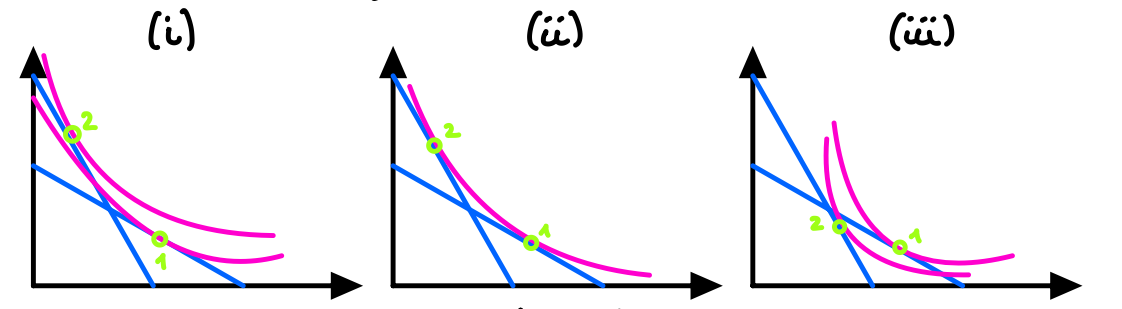
\includegraphics[width=\textwidth]{images/2015_16_1.png}
\end{figure}

\underline{Case 3:} ( $\left.p<p^{\text {aut }}\right)$

Substitute $A$ sells 1 and buys 1 in case 2. The argument is just the inverse.

For agent $B$ the argument is always just the inverse in all cases.

We see that at least one agent is weakly better off.
}
{
\subsubsection*{Exercise 2}

\begin{enumerate}[label=(\alph*)]
{\item
Since $A$ cares more about $x_{1}$ and $B$ more about $x_{2}$, the PE allocations ce around the edges of the box (in blue).

$$
P E=\left\{x_{2}^{A}=0 \text{ or } x_{1}^{B}=0\right\}
$$

\begin{figure}[!h]
    \centering
    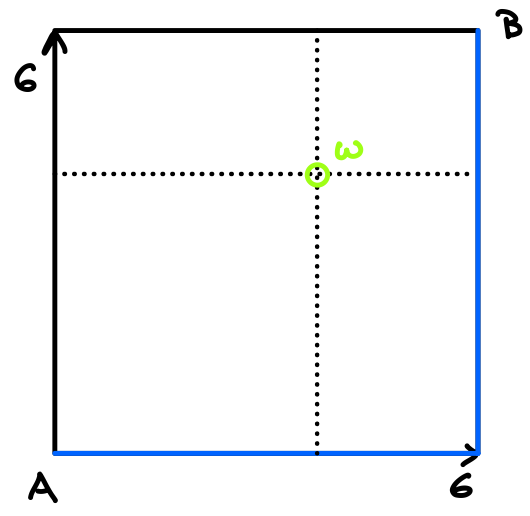
\includegraphics[width=.5\textwidth]{images/2015_16_2.png}
\end{figure}
}
{\item
For PE, equate MRS across agents:

$$
\operatorname{MRS}^{A}=2 \stackrel{!}{=} \operatorname{MRS}^{B}=\frac{x_{2}^{B}}{x_{1}^{B}} \Leftrightarrow x_{2}^{B}=2 x_{1}^{B}
$$

For $C E$ consumers behave optimally \& markets must clear. Let $p=p_{1} / p_{2}$

A: By linearity of preferences:

$$
x_{1}^{A}=\left\{\begin{array}{lll}
    \infty & \text {if } p<2 \\
    \mathbb{R}^{+} & \text {if } p=2 \\
    0 & \text {if } p>2
\end{array} \quad x_{2}^{A}=\left\{\begin{array}{lll}
    \infty & \text {if } p>2 \\
    \mathbb{R}^{+} & \text {if } p=2 \\
    0 & \text {if } p<2
\end{array}\right.\right.
$$

B:

\begin{align*}
    \max _{C_{1}^{8}, c_{2}^{8}} \ln \left(x_{1}^{8}\right)+\ln \left(x_{2}^{8}\right) \\
    \text{s.t. } p x_{1}^{B}+x_{2}^{B}=p^{2}+2
\end{align*}

FOCs

\begin{align*}
    &\frac{1}{x_{1}^{B}}-\lambda p=0 \\
    &\frac{1}{x_{2}^{B}}-\lambda=0 \\
    \Longrightarrow \quad & x_{2}^{B}=x_{1}^{B} p
\end{align*}

Plug into $B C$ :

$$
x_{1}^{B}=\frac{p+1}{p} ; x_{2}^{B}=p+1
$$

\underline{Market Clearing: } 

For markets to clear we have $p=2$. Otherwise $A$ will have infinite demand for one of the goods:

$$
\begin{gathered}
x_{1}^{B}=\frac{3}{2} ;\quad x_{2}^{B}=3 \\
x_{1}^{A}=6-x_{1}^{3}=\frac{9}{2} ;\quad x_{2}^{A}=6-x_{2}^{B}=3
\end{gathered}
$$

\underline{Competitive Equilibrium: }

\begin{align*}
    \left(x_{1}^{A}, x_{2}^{A}\right) &= (\frac{9}{2},3) \\
    \left(x_{1}^{B}, x_{2}^{B}\right) &= (\frac{3}{2},3) \\
    p&=2
\end{align*}

It is $P E$ since $x_{2}^{B}=3=p x_{1}^{B}=2\frac{3}{2}$.
}
\end{enumerate}
}
{
\subsubsection*{Exercise 3} 

$$
w^{A}=(8,4) ; w^{B}=(2,4)
$$

\begin{enumerate}[label=(\alph*)]
{\item
$$
\begin{aligned}
& M R S^{A}=\frac{1 / 2}{1 / 2}=1 \stackrel{!}{=} MRS^{B}=\frac{1 / 2}{1 / 2} \frac{\frac{\partial u^{B}(\cdot)}{\partial x_{1}}}{\frac{\partial u^{B}(\cdot)}{\partial x_{2}}} \\
& \Longleftrightarrow \frac{\partial u^{B} \left(\cdot\right)}{\partial x_{1}}=\frac{\partial u^{B}(\cdot)}{\partial x_{2}} \Longleftrightarrow x_{1}^{B}=x_{2}^{B}
\end{aligned}
$$

PE in blue. Defined by

$$
x_{2}^{B}=\left\{\begin{array}{ll}
x_{1}^{B} & \text { if } x_{1}^{B} \leq 8 \\
8 & \text { else }
\end{array}\right\}
$$

\begin{figure}[!h]
    \centering
    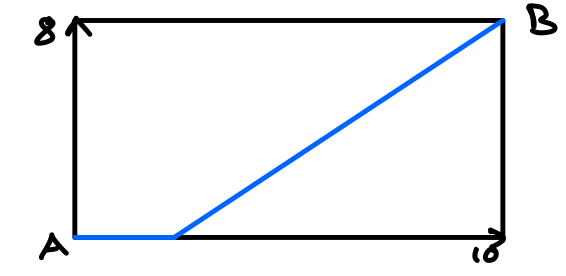
\includegraphics[width=.5\textwidth]{images/2015_16_3.png}
\end{figure}
}
{\item 
Budget constraints:

\begin{align*}
    \text{at } t = 0: \quad & q_1 \theta_1^h+q_2 \theta_2^h=0 \\
    \text{at } t = 1: \quad & x_1^h=w_1^h+\theta_1^h \\
    & x_2^h=w_2^h+\theta_2^h
\end{align*}

Plug the $\theta$s into first BC:

$$
q_{1}\left(x_{1}^{h}-w_{1}^{h}\right)+q_{2}\left(x_{2}^{h}-w_{2}^{h}\right)=0
$$

UMP:

$$
\begin{aligned}
& \max _{x_{1}^{h}, x_{2}^{h}} \quad \pi_{1} u^{h}\left(x_{1}^{h}\right)+\pi_{2} u^{h}\left(x_{2}^{h}\right) \\
& \text { s.t. } q_{1}\left(x_{1}^{h}-w_{1}^{h}\right)+q_{2}\left(x_{2}^{h}-w_{2}^{h}\right)=0
\end{aligned}
$$

FOCs:

\begin{align*}
    \pi_{1} \frac{\partial u^{h}(\cdot)}{\partial x_{1}^{h}}-\lambda q_{1}=0 \\
    \pi_{2} \frac{\partial u^{h}(\cdot)}{\partial x_{2}^{h}}-\lambda q_{2}=0 \\
    \longrightarrow \frac{q_{1}}{q_{2}}=\frac{\pi_{1}}{\pi_{2}} \frac{\partial u^{h}(\cdot)}{\partial x_{1}^{h}}\left(\frac{\partial u^{h}(\cdot)}{\partial x_{2}^{h}}\right)^{-1} \tag{I}
\end{align*}

\underline{Agent A:}

By $\pi_{1}=\pi_{2}$ \& linearity:

\begin{align*}
    \frac{q_{1}}{q_{2}}=1
\end{align*}

\underline{Agent B:}

Plug $\frac{q_{1}}{q_{2}}=1$ into (I) and also $\pi_{1}=\pi_{2}$ :

\begin{equation*}
    \frac{\partial u^{B}(\cdot)}{\partial x_{1}^{B}}=\frac{\partial u^{B}(\cdot)}{\partial x_2^{B}} \Leftrightarrow x_{1}^{B}=x_{2}^{B} \tag{II}
\end{equation*}

Plug (II) into $B C$ of $B$ using $\frac{q_{1}}{q_{2}}=1$ :

$$
x_{1}^{B}=x_{2}^{B}=\frac{w_{1}^{B}+w_{2}^{B}}{2}=3
$$

\underline{Market Clearing: }

$$
\begin{aligned}
& x_{1}^{A} \stackrel{!}{=} w_{1}^{A}+w_{1}^{B}-x_{1}^{B}=7 \\
& x_{2}^{A} \stackrel{!}{=} w_{2}^{A}+w_{2}^{B}-x_{2}^{B}=5
\end{aligned}
$$

\underline{Competitive Equilibrium: }

$$
\begin{aligned}
\left(x_{1}^{A}, x_{2}^{A}\right) & =(7,5) \\
\left(x_{1}^{B}, x_{2}^{B}\right) & =(3,3) \\
\frac{q_{1}}{q_2} & =1
\end{aligned}
$$

It is PE as $x_{1}^{B}<8$ and $x_{2}^{B}=x_{1}^{B}$.
}
{\item 
By (I) we know that $\frac{q_{1}}{q_{2}}>1$. Thus insurance for $B$ is more expensive $\&$ she buys less of it. At the same time, $A$ believes $s=1$ to be more likely. Therefore, $A$ consumes more in $s=1$, and $B$ less. A consumes less in $s=2, B$ consumes more.
}
\end{enumerate}
}\newpage
\section{Macroeconomics Final 2016 / 17}

{
\subsection*{Exercise 1}

\begin{enumerate}[label=(\alph*)]
{\item 
True

The DIS is given by

$$
\tilde{y}_{t}=\frac{1}{\sigma}\left(i_{t}-\mathbb{E}_{t}\left(\pi_{t+1}\right)-r_{t}^n\right)+\mathbb{E}_{t}\left(\tilde{y}_{t+1}\right)
$$

The $C B$ can influence $i_t$ which indirectly has an effect on $\mathbb{E}_{t}\left(\pi_{t+1}\right)$ as long as current and future inflation are linked. Even more so if the $C B$ can commit to a policy.
}
{
\item 
False

They depend on the nominal rate. And the nominal rate depends on inflation.
}
{
\item 
False 

Output increases but real wages actually increase since $\omega_{t}=w_{t}-p_{t}=\sigma c_{t}+n_{t}$ and in equilibrium $c_{t}=y_{t}$. Therefore, higher $y_{t}$ implies higher real wages. (reference: slide deck 3, p. 37)
}
{
\item 
True

Unless there are "menu costs". Output gap fluctuations still cause welfare losses.
}
\end{enumerate}
}
{
\subsection*{Exercise 2}

\begin{enumerate}[label=(\alph*)]
{\item 
$u_t$ represents an exogenous shock that affects marginal costs. 
E.g. a pandemic causing supply-chains to break down. Since $u_{t}$ follows on AR (1) process, the shocks are persistent over time.

The addition of $u_{t}$ in this model "breaks" the divine coincidence: the $C B$ cannot stabilize output by only focusing on stabilizing prices.
}
{
\item 
Conjectures:

\begin{align}
    & \pi_{t}=\psi_{\pi} u_{t} \tag{I} \\
    & x_{t}=\psi_{x} u_{t} \tag{II}
\end{align}

Plug (I), (II) \& interest rate rule into (1) \& (2):

$$
\begin{aligned}
& \left|\begin{array}{l}
\psi_{\pi} u_{t}=\beta \mathbb{E}_{t}\left(\psi_{\pi} v_{t+1}\right)+\kappa \psi_{x} u_{t}+u_{t} \\
\psi_{x} u_{t}=\mathbb{E}_{t}\left(\psi_{x} v_{t+1}\right)-\left(\Phi_{\pi} \psi_{\pi} u_{t}-\mathbb{E}_{t}\left(\psi_{\pi} u_{t+1}\right)\right)
\end{array}\right| \\
& \Leftrightarrow\left|\begin{array}{l}
\psi_{\pi}=\beta \psi_{\pi} \rho_{u}+\kappa \psi_{x}+1 \\
\psi_{x}=\psi_{x} \rho_{u}-\phi_{\pi} \psi_{\pi}+\psi_{\pi} \rho_{u}
\end{array}\right| \\
& \Leftrightarrow \left\lvert\, \begin{array}{l}
\psi_{\pi}\left(1-\beta \rho_{u}\right)=\kappa \psi_{x}+1 \\
\psi_{x}\left(1-\rho_{u}\right)=\left(\rho_{u}-\phi_{\pi}\right) \psi_{\pi}
\end{array}\right. \\
& \Longrightarrow \psi_{\pi}\left(1-\beta \rho_{u}\right)=\kappa \frac{\rho_{u}-\phi_{\pi}}{1-\rho_{u}} \psi_{\pi}+1 \\
& \Leftrightarrow \psi_{\pi}\left(1-\beta\rho_{u}-\kappa \frac{\rho_{u}-\phi_{\pi}}{1-\rho_{u}}\right)=1 \\
& \pi_{t}=\frac{1-\rho_{u}}{\left(1-\beta\rho_{u}\right)\left(1-\rho_{u}\right)-\kappa\left(\rho_{u}-\varnothing_{\pi}\right)} u_{t} \\
& x_{t}=\frac{\rho_{u}-\phi_{\pi}}{\left(1-\beta \rho_{u}\right)\left(1-\rho_{u}\right)-\kappa\left(\rho_{u}-\varnothing_{\pi}\right)} u_{t} \\
& \operatorname{Var}\left(x_{t}\right)=\psi_{x}^{2} \operatorname{Var}\left(u_{t}\right) \\
& \Rightarrow \frac{\partial \operatorname{Var}\left(x_{t}\right)}{\partial \phi_{\pi}}<0
\end{aligned}
$$

Volatility increases, the weaker $C B$ reacts to $\pi_{t}$. Because divine coincidence is broken!

\color{red} No (c) or (d)? \color{black}
}
{
\item[(e)]

$$
\begin{aligned}
\min _{\phi_{\pi}} L\left(\phi_{\pi}\right) &=\operatorname{Var}\left(\pi_{t}\right)+\vartheta \operatorname{Var}\left(x_{t}\right) \\
& =\left(\psi_{\pi}^{2}+\vartheta \psi_{x}^{2}\right) \operatorname{Var}\left(u_{t}\right) 
\end{aligned}
$$
%%% from here
FOC:

$$
\begin{aligned}
& 0 = 2 \psi_{\pi} \frac{\partial \psi_{\pi}}{\partial \phi_{\pi}}+2 \vartheta \psi_{x} \frac{\partial \psi_{x}}{\partial \phi_{\pi}} \\
0=&\left(1-\rho_{u}\right)\left(-\left(1-\rho_{u}\right) \kappa \right) \\
& +\vartheta\left(\rho_{u}-\phi_{\pi}\right)\left(\kappa\left(\rho_{u}-\phi_{\pi}\right)-\left(1-\beta\rho_{ u}\right)\left(1-\rho_{u}\right)-\left(\rho_{u}-\phi_{\pi}\right) \kappa\right) \\
& \left(1-\rho_{u}\right)^{2} \kappa=-\vartheta\left(\rho_{u}-\phi_{\pi}\right)\left(1-\beta\rho_{u}\right)\left(1-\rho_{u}\right) \\
& \rho_{u}-\phi_{\pi}=\frac{1-\rho_{u}}{1-\beta\rho_{u}} \frac{\kappa}{\vartheta} \\
& \phi_{\pi}=\rho_{u}+\frac{\kappa}{\vartheta} \frac{1-\rho_{u}}{1-\beta\rho_{u}}
\end{aligned}
$$

Note, that $\rho_{u}=0$ implies $\phi_{\pi}=\frac{\kappa}{\theta}$. 

At the same time $\rho_{u}=1$ implies $\phi_\pi=1$.
}
\end{enumerate}
}\newpage
\section{Econometrics Final 2017 / 18}

{
\subsection*{Watson}

{
\subsubsection*{Exercise 1}

\begin{enumerate}[label=(\alph*)]
{\item 
$$
\begin{aligned}
\mathbb{E}_{t}\left(Y_{t+1} \mid \varepsilon_{t}+\varepsilon_{t-1}=2\right) & =\mathbb{E}_{t}\left(\varepsilon_{t+1}+0.8 \varepsilon_{t} \mid \varepsilon_{t}=2-\varepsilon_{t-1}\right) \\
& =\mathbb{E}_{t}\left(\varepsilon_{t+1}+0.8\left(2-\varepsilon_{t-1}\right)\right) \\
& =\mathbb{E}_{t}\left(\varepsilon_{t+1}\right)+1.6-0.8 \mathbb{E}_{t}\left(\varepsilon_{t-1}\right) \\
& =1.6
\end{aligned}
$$

The optimal forecast is the conditional expectation of $Y_{t+1}$ given the information that $\varepsilon_{t}+\varepsilon_{t-1}=2$.
}
{\item 
$$
\begin{aligned}
\hat{\phi} &= \frac{\widehat{\operatorname{Cov}}\left(Y_{t}, Y_{t-1}\right)}{\widehat{\operatorname{Var}}\left(Y_{t-1}\right)} \\
\xrightarrow{p} \frac{\operatorname{Cov}\left(Y_{t}, Y_{t-1}\right)}{\operatorname{Var}\left(Y_{t-1}\right)} & =\frac{\operatorname{Cov}\left(\varepsilon_{t}+0.8 \varepsilon_{t-1}, \varepsilon_{t-1}+0.8 \varepsilon_{t-2}\right)}{\operatorname{Var}\left(\varepsilon_{t-1}+0.8 \varepsilon_{t-2}\right)} \\
& =\frac{\operatorname{Var}\left(\varepsilon_{t-1}\right) \cdot 0.8}{\operatorname{Var}\left(\varepsilon_{t-1}\right)+0.64 \operatorname{Var}\left(\varepsilon_{t-2}\right)} \\
& =\frac{0.8}{1.64}=0.488
\end{aligned}
$$
}
\end{enumerate}
}
{
\subsubsection*{Exercise 2}

\begin{enumerate}[label=(\alph*)]
{\item 
It is not invertible. Let $X_{t}=Y_{t}-\beta$, then

$$
\begin{aligned}
X_{t} & =\varepsilon_{t}-\theta \varepsilon_{t-1} \\
\Leftrightarrow \varepsilon_{t} & =X_{t}+\theta \varepsilon_{t-1} \\
& =X_{t}+\theta\left(X_{t-1}+\theta \varepsilon_{t-2}\right) \\
& \quad \vdots \\
& =\theta^{t} \varepsilon_{0}+\sum_{i=0}^{t-1} \theta^{i} X_{t-i}
\end{aligned}
$$

If $|\theta| \geq 1$, then $\theta^{t} \varepsilon_{0}$ does not converge towards zero as $t$ gets large. Therefore, $X_{t}$ cannot be expressed only by its lagged values plus the period $t$ error.
}
{\item 
$$
\begin{aligned}
\sqrt{T}(\bar{Y}-\beta) & =\sqrt{T} \frac{1}{T} \sum_{t=1}^{T}\left(Y_{t}-\beta\right)=\frac{1}{\sqrt{T}} \sum_{t=1}^{T}\left(\varepsilon_{t}-\theta \varepsilon_{t-1}\right) \\
& =\frac{1}{\sqrt{T}}\left(\sum_{t=1}^{T} \varepsilon_{t}-\theta \sum_{t=0}^{T-1} \varepsilon_{t}\right)
\end{aligned}
$$

$$
\begin{aligned}
& =\frac{1}{\sqrt{T}}\left(\sum_{t=1}^{T} \varepsilon_{t}-\theta \sum_{t=1}^{T} \varepsilon_{t}-\theta \varepsilon_{0}+\theta \varepsilon_{T}\right) \\
& =\underbrace{(1-\theta) \frac{1}{\sqrt{T}} \sum_{t=1}^{T} \varepsilon_{t}}_{\xrightarrow{d} N(0,\sigma^2(1-\theta)^2)}+\underbrace{\frac{\theta}{\sqrt{T}}\left(\varepsilon_{T}-\varepsilon_{0}\right)}_{\xrightarrow{p}0}
\end{aligned}
$$

Apply Slutsky:

$$
\begin{aligned}
& \sqrt{T}(\bar{Y}-\beta) \xrightarrow{d} N\left(0, \sigma^{2}(1-\theta)^{2}\right) \\
& \sqrt{T}(\bar{Y}-\beta) \xrightarrow{d} N(0,1)
\end{aligned}
$$
}
{\item 
Delta method: $g(x)=x^{2} ;\left(g^{\prime}(x)\right)^{2}=4 x^{2}$

$$
\sqrt{T}\left(\bar{Y}^{2}-\beta^{2}\right) \xrightarrow{d} N\left(0,1 \cdot g^{\prime}(\beta)^{2}\right)
$$

Use $g^{\prime}(\beta)^{2}=4 \beta^{2}$ and $\beta=5$. Then:

$$
\sqrt{T}\left(\bar{Y}^{2}-25\right) \xrightarrow{d} N\left(0,100\right)
$$
}
{\item 
If $\theta=1$, this would lead to $V=0$ which is clearly incorrect. There, I would do the following:

$$
\begin{aligned}
Y_{t}-\beta & =u_{t}=\varepsilon_{t}-\varepsilon_{t-1} \\
\frac{1}{\sqrt{T}} \sum Y_{t}-\beta & =\frac{1}{\sqrt{T}} \sum_{t=1}^{T} u_{t}
\end{aligned}
$$

Now $u_{t} \sim N(0,2)$ but not iid anymore.

\color{red} How further?? \color{black}
}
\end{enumerate}
}
{
\subsubsection*{Exercise 3}

\begin{enumerate}[label=(\alph*)]
{\item 
$$
\begin{aligned}
& \bar{X}_{t}=\frac{1}{n} \sum_{i=1}^{n} \xi_{t}+\varepsilon_{i t}=\xi_{t}+\frac{1}{n} \sum_{i=1}^{n} \varepsilon_{i t} \\
& \xi_{t} \xrightarrow{p} \xi_{t} \text { as } \xi_{t}=\xi_{t} \\
& \frac{1}{n} \sum_{i=1}^{n} \varepsilon_{t} \xrightarrow{p} \mathbb{E}\left(\varepsilon_{i t}\right)=0 \text { by LLN}
\end{aligned}
$$

I conclude that

$$
\bar{X}_{t} \longrightarrow \xi_{t}
$$
}
{\item 
$$
\begin{aligned}
M S E & =\mathbb{E}\left(\left(\bar{X}_{t}-\xi_{t}\right)^{2}\right) \\
& =\mathbb{E}\left(\left(\frac{1}{n} \sum_{i=1}^n \varepsilon_{i t}\right)^{2}\right)=\left(\frac{1}{n}\right)^{2} \mathbb{E}\left(\sum_{i=1}^{n} \varepsilon_{i t}^{2}+\sum_{j \neq i} \varepsilon_{i t} \varepsilon_{j t}\right) \\
& =\frac{1}{n^{2}} \sum_{i=1}^{n} \underbrace{\mathbb{E}\left(\varepsilon_{it}^{2}\right)}_{\sigma^{2}=1}+\sum_{j \neq i} \underbrace{\mathbb{E}\left(\varepsilon_{i t} \varepsilon_{j t}\right)}_{=0 \text { by iid } N(0,1)} \\
& =\frac{1}{n}
\end{aligned}
$$
}
{\item 
\color{red} Maybe MLE-estimator? \color{black}
}
\end{enumerate}
}
}

\newpage
{
\subsection*{Honor\'e}

{
\subsubsection*{Exercise 1}

\begin{enumerate}[label=(\alph*)]
{\item 
$C I=[\hat{\beta} \pm 1.96 \cdot \hat{SE}(\hat{\beta})] \cong[0.227 ; 0.962]$
}
{\item 
Reject the hypothesis:

$$t=\frac{\hat{\beta}-\beta_{0}}{\hat{SE}(\hat{\beta})}=\frac{0.092+0.2}{0.115}=2.545>1.96$$
}
{\item 
$$
\begin{aligned}
x_{i}^{\prime} \beta & =1.1 \cdot 0.98+0.8 \cdot 0.152+1 \cdot(-0.223)-1.872 \\
& =-0.896 \\
P\left(y_{i} =1 | x_{i}\right)&=\frac{\exp \left(x_{i}^{\prime} \beta\right)}{1+\exp \left(x_{i}^\prime \beta\right)} \cong 28.993 \%
\end{aligned}
$$
}
{\item 
$$
\begin{aligned}
\frac{\partial P\left(y_{i}=1 \mid x_{i}\right)}{\partial b l o o d p} & =P\left(y_{i}=1 \mid x_{i}\right) P\left(y_{i}=0 \mid x_{i}\right) \cdot \beta_{\text {bloodp }} \\
& \cong 0.202
\end{aligned}
$$
}
\end{enumerate}
}
{
\subsubsection*{Exercise 2}

\begin{enumerate}[label=(\arabic*)]
{\item 
$$
\begin{aligned}
\sqrt{n}(\hat{\beta}-\beta) &\xrightarrow{d} N\left(0, A^{-1} B A^{-1}\right) \\
A &=\mathbb{E}\left(\left(1+2 \beta x_{i}\right)^{2}\right)\\
B &=\sigma^{2} \mathbb{E}\left(\left(1+2 \beta x_{i}\right)^{2}\right)
\end{aligned}
$$

Thus, we can simplify:

$$
\sqrt{n}(\hat{\beta}-\beta) \xrightarrow{d} N\left(0, \sigma^{2} \mathbb{E}\left(\left(1+2 \beta x_{i}\right)^{2}\right)^{-1}\right)
$$
}
{\item 
$$
\begin{aligned}
\sqrt{n}(\hat{\beta}-\beta) &\xrightarrow{d} N\left(0, G^{-1} S G^{-1}\right) \\
G &= \mathbb{E}\left(-x_{i}\left(1+2 \beta x_{i}\right)\right)=-\left(\mathbb{E}\left(x_{i}\right)+2 \beta \mathbb{E}\left(x_{i}^{2}\right)\right) \\
S &= V\left(\left(y_{i}-\left(\beta+\beta^{2} x_{i}\right)\right) x_{i}\right)=V\left(\varepsilon_{i} x_{i}\right) \\
&= \mathbb{E}\left(\varepsilon_{i}^{2} x_{i}^{2}\right)-\mathbb{E}\left(\varepsilon_{i} x_{i}\right)^{2}=\mathbb{E}\left(\mathbb{E}\left(\varepsilon_{i}^{2} \mid x_{i}\right) x_{i}^{2}\right) \\
&= \sigma^{2} \mathbb{E}\left(x_{i}^{2}\right)
\end{aligned}
$$
}
{\item 
$$
\begin{aligned}
& \sqrt{n}(\hat{\beta}-\beta) \xrightarrow{d} N\left(0, \left(G^{\prime} S^{-1} G\right)^{-1}\right) \\
& G=\mathbb{E}\left[\begin{array}{l}
-\left(1+2 \beta x_{i}\right) \\
-x_{i}\left(1+2 \beta x_{i}\right)
\end{array}\right] \\
& S=V\left[\begin{array}{ll}
\varepsilon_{i} \\
\varepsilon_{i} x_{i}
\end{array}\right]=\mathbb{E}\left[\begin{array}{ll}
\varepsilon_{i}^{2} & \varepsilon_i^{2} x_{i} \\
\varepsilon_{i}^{2} x_{i} & \varepsilon_{i}^{2} x_{i}^{2}
\end{array}\right]=\sigma^{2}\left[\begin{array}{ll}
1 & \mathbb{E}\left(x_{i}\right) \\
\mathbb{E}\left(x_{i}\right) & \mathbb{E}\left(x_{i}^{2}\right)
\end{array}\right]
\end{aligned}
$$
}
\end{enumerate}
}
{
\subsubsection*{Exercise 3}

\begin{itemize}
\item When we think that the treatment is that some variable $x$ is greater then some threshold $c$. Examples would be:
\begin{itemize}
    \item let $x$ be time, $c$ be the year 1989, and $y$ is GDP growth in eastern Germany. Since before $c$, eastern Germany was under communist rule, one could interpret 1989 as the threshold after which the treatment "capitalism" was implemented.
    \item let $x$ be school grades, $c$ be the cutoff to get into med-school, and $y$ be earnings. We can use this cut-off as a treatment.
\end{itemize}
\item It assumes, that the regressions in the counterfactual would continue continuously. Also, that the treatment at $c$ actually causes a jump in $y$.
\end{itemize}

The following graph helps to drive the idea home:

\begin{figure}[!htp]
    \centering
    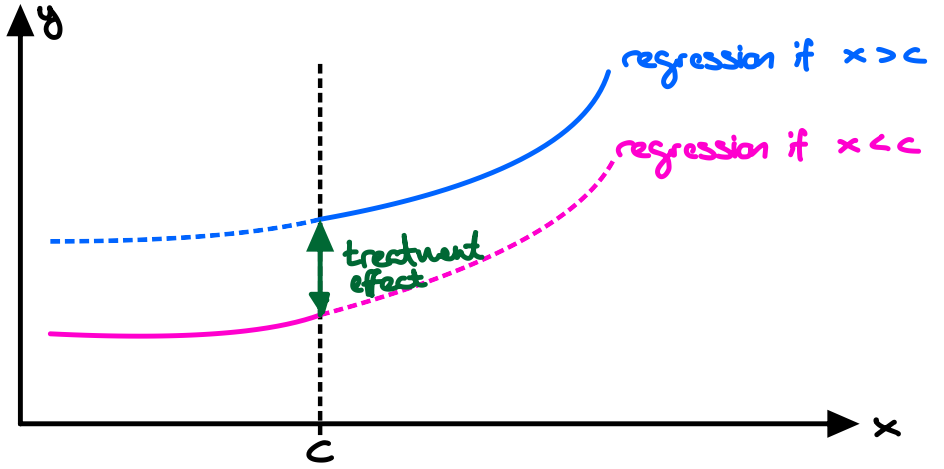
\includegraphics[width=\textwidth]{images/2017_18.png}
\end{figure}
}
{
\FloatBarrier
\subsubsection*{Exercise 4}

First, we get rid of the $\alpha_{i}$ by taking first differences:

$$
\Delta y_{i t}=\Delta x_{i t} \beta_{1}+\Delta x_{2i t} \beta_{2}+\Delta \varepsilon_{i t} \quad t=2,3
$$

Note, that we can use the following to find the moment conditions:

$$
\begin{aligned}
\mathbb{E}\left(\Delta \varepsilon_{i t} \mid x_{1is}\right)=0 & \quad \forall t,s \\
\mathbb{E}\left(\Delta \varepsilon_{i t} \mid x_{2 i s}\right)=0 & \quad \forall t \geq s
\end{aligned}
$$

$$
\begin{aligned}
\text{for }x_{1 i t}: \quad & \mathbb{E}\left(\Delta \varepsilon_{i t} x_{1 i s}\right)=0 \quad \forall s, t \\
&\mathbb{E}\left(\Delta y_{i t}-\Delta x_{1i t} \beta_{1}+\Delta x_{2 it} \beta_{2}\right) x_{1 i s}=0 \quad \forall s, t \\
&\longrightarrow 6 \text{ moment conditions} \\
\text{for }x_{2 i t}: \quad & \mathbb{E}\left(\Delta \varepsilon_{i t} x_{2is}\right)=0 \quad \forall (s, t) \in\{(1,2),(1,3),(2,3)\} \\
&\mathbb{E}\left(\left(\Delta y_{i t}-\Delta x_{1 i t} \beta_{1}+\Delta x_{2i t} \beta_{2}\right) x_{2 i s}\right)=0 \quad \forall (s, t) \in\{(1,2),(1,3),(2,3)\} \\
&\longrightarrow 3 \text{ moment conditions}
\end{aligned}
$$

Therefore, we can use 9 moment conditions in total, and GMM will work to estimate $\left(\beta_{1}, \beta_{2}\right)$.
}
}
\newpage
\section{Macroeconomics Final 2018 / 19}

{
\subsection*{Exercise 1}

\begin{enumerate}[label=(\alph*)]
{\item 
False

We showed in class that in this case, the optimal interest rate is zero. Together with the result of the representative consumer behaviour:

$$
\pi=i_{t}-\rho=-\rho
$$

I.e. constant deflation at rate $\rho$.
}
{
\item 
False

We analyzed the following welfare loss:

$$
W=-\mathbb{E}_{0} \sum_{t=0}^{\infty} \beta^{t} \frac{U_{t}-U}{U_{c} C}
$$

And looked at a 2nd order Taylor approximation:

$$
W \approx \frac{1}{2} \mathbb{E}_{0} \sum_{t=0}^{\infty} \beta^{t}\left(-\Phi \hat{x}_{t}+\left(G+\frac{\varphi+\alpha}{1-\alpha}\right) \hat{x}_{t}^{2}+\frac{\varepsilon}{\lambda} \pi_{t}^{2}\right)+t . i . \rho \text {. }
$$

Note, that $\pi_{t}$ does enter the welfare loss such that $\pi_{t}=0$ would lead to minimal welfare losses.
}
{
\item 
True

We have seen that with a distortional labour income tax, the divine coincidence breaks down. This means, inflation targeting is insufficient to stabilize outcome.

More specifically in exercise 2, PS3, we found the following NKPC:

$$
\pi_{t}=\beta \mathbb{E}_{t}\left(\pi_{t+1}\right)+\lambda(1+\varphi) x_{t}+\lambda\left(\mu+\tau_{t}\right)
$$
}
{
\item 
True.

It is only attainable if the natural real wage does not change, i.e. is constant.
}
\end{enumerate}
}
{
\subsection*{Exercise 2}

\begin{enumerate}[label=(\alph*)]
{\item 
$$
\max _{N_{t}}\left(P_{t}-1\right) N_{t}
$$

This implies

$$
N_{t}=\left\{\begin{array}{lll}
\infty & \text { if } & P_{t} > 1 \\
\mathbb{R}^{+} & \text { if } & P_{t}=1 \\
0 & \text { if } & P_{t}<1
\end{array}\right.
$$

Therefore, we may conclude that $P_{t}=1$, and the firm employs everyone that wants to work.
}
{
\item 
First, obtain labour supply by solving

$$
\begin{aligned}
& \max \mathbb{E}_{0}\left[\sum_{t=0}^{\infty} \beta^{t}\left(C_{t}-\frac{N_{t}^{1+\varphi}}{1+\varphi}\right)\right] \\
& \text { s.t. } 0=B_{t-1}+M_{t-1}+N_{t}-P_{t} C_{t}-Q_{t} B_{t}-M_{t}
\end{aligned}
$$

Classic result from FOCs:

$$
\begin{aligned}
& N_{t}^{\varphi}=\frac{W_{t}}{P_{t}}=1 \\
\Rightarrow & N_{t}=1
\end{aligned}
$$

Thus, labour supply is 1 , and this is the maximum that can be produced. Use CIA \& market clearing:

$$
G_{t}=Y_{t}=\frac{M_{t}}{Z_{t}}
$$

We conclude that:

$$
Y_{t}=\min \left\{\frac{M_{t}}{Z_t}, 1\right\}
$$
}
{
\item 
The positive shock impacts the CIA constraint. Increase in money demanded per unit of consumption. If supply does not increase (e.g. because $N_{t}=1$ is hit), need to reduce consumption, and lower output.
}
{
\item 
Social planner problem:

$$
\begin{aligned}
\max & \mathbb{E}_{0}\left[ \sum_{t=0}^{\infty} \beta^{t}\left(C_{t}-\frac{N_{t}^{1+\varphi}}{1+\varphi}\right)\right] \\
\text { s.t. } & C_{t}=Y_{t}=N_{t}
\end{aligned}
$$

Plug constraint into objective function:

$$
\max _{N_{t}} \mathbb{E}_{0}\left[\sum_{t=0}^{\infty} \beta^{t}\left(N_{t}-\frac{N_{t}^{1+\varphi}}{1+\varphi}\right)\right]
$$

FOC:

$$
1-N_{t}^{\varphi}=0 \Leftrightarrow N_{t}=1
$$

By production technology:

$$
Y_{t}^{e}=1
$$

Use $Y_{e}=1, P_{t}=1$ in CIA constraint:

$$
M_{t}=Z_{t}
$$

I.e. the money supply reacts to $Z_t$.
}
{
\item 
No. Both short- and long-run $Y_{t}=\min \left\{\frac{M_{t}}{Z_{t}}, 1\right\}$.

Here, prices and wages are fixed, and there is a persistent effect of money on output.

In NK model, both prices \& wages can be adjusted.
}
\end{enumerate}
}
\newpage
\section{Microeconomics Midterm 2019 / 20}

{
\subsection*{Schmidt}

{
\subsubsection*{Exercise 1}

\begin{enumerate}[label=(\roman*)]
{\item 
First, find incomes:

$$
w^{0}=42 \quad w^{1}=36 \quad w^{2}=50
$$

Look for violations of WARP:

\begin{table}[!htp]
    \centering
    \begin{tabular}{|c|c|l|l|l|l|}
    \hline
    $t$ & $t^{\prime}$ & $p^{t} x^{t^{1}}$ & $\sum$ & $w^{t}$ & revealed preferences \\
    \hline \multirow{2}{*}{0} & 1 & $p^{0} x^{1}=48$ & $>$ & 42 & - \\
    \cline { 2 - 6 } & 2 & $p^{0} x^{2}=40$ & $<$ & 42 & $x^{0}>x^{2}$ \\
    \hline \multirow{2}{*}{1} & 0 & $p^{1} x^{0}=33$ & $<$ & 36 & $x^{1}>x^{0}$ \\
    \cline { 2 - 6 } & 2 & $p^{1} x^{2}=39$ & $>$ & 36 & - \\
    \hline \multirow{2}{*}{2} & 0 & $p^{2} x^{0}=52$ & $>$ & 50 & - \\
    \cline { 2 - 6 } & 1 & $p^{2} x^{1}=48$ & $<$ & 50 & $x^{2}>x^{1}$ \\
    \hline
    \end{tabular}
\end{table}

From the table we see that we never have $p^{t} x^{t^{\prime}} \leq w^{t}$ and $p^{t^{\prime}} x^{t} \leq w^{t^{\prime}}$. Therefore, WARP is satisfied.
}
{\item 
From the last row we have $x^{0}>x^{2}$ and $x^{2}>x^{1}$

Transitivity implies $x^{0}>x^{\prime}$ but we found the opposite: $x^{\prime}>x^{0}$. Therefore, transitivity is violated.
}
\end{enumerate}
}
{
\subsubsection*{Exercise 2}

\begin{enumerate}[label=(\alph*)]
{\item 
Consumer 1: at optimum $e_{1}(\cdot)=w_{1}$ \& $u_{1}=v_{1}(\cdot)$

$$
\begin{aligned}
w_{1} & =v_{1}\left(p, w_{1}\right) \sqrt{p_{1} p_{2}} \\
\Leftrightarrow v_{1}\left(p, w_1\right) & =\frac{w_{1}}{\sqrt{p_{1} p_{2}}}
\end{aligned}
$$

Use Roy's identity:

$$
\begin{aligned}
x_{1}^1(p, w) & =-\frac{\frac{\partial v_{1}\left(p_{1} w\right)}{\partial p_{1}}}{\frac{\partial v_{1}\left(p_{1} w\right)}{\partial w_{1}}}=-\frac{-\frac{1}{2} \frac{w_{1}}{\sqrt{p_{2}} p_{1}^{-3 / 2}}}{\frac{1}{\sqrt{p_{1} p_{2}}}} \\
& =\frac{w_{1}}{2 p_{1}}
\end{aligned}
$$

By symmetry: $x_{2}^1\left(p_{1} w\right)=\frac{w_{1}}{2 p_{2}}$

Consumer 2: Transform utility function.

$$
u_{2}\left(x_{1}, x_{2}\right)=x_{1}^{\frac{3}{3+a}} x_{2}^{\frac{a}{3+a}}
$$

This is standard Cobb-Dauglas:

$$
x_{1}^{2}(p, w)=\frac{3}{3+a} \frac{w_{2}}{p_{1}} ; x_{2}^1 (p, w)=\frac{a}{3+a} \frac{w_{2}}{p_{2}}
$$
}
{\item 
Good 1: $\quad x_{1}^{1}+x_{1}^{2}=\frac{1}{p_{1}}\left[\frac{1}{2} w_{1}+\frac{3}{3+a} w_{2}\right]$

$$
\longrightarrow \frac{1}{2}=\frac{3}{3+a} \Longleftrightarrow a=3
$$

Good 2: $x_{2}^{1}+x_{2}^{2}=\frac{1}{p_{2}}\left[\frac{1}{2} w_{1}+\frac{a}{3+a} w_{2}\right]$

$$
\longrightarrow \frac{1}{2}=\frac{a}{3+a} \Longleftrightarrow a=3
$$

Thus $a=3$ solves the problem for both goods.
}
\end{enumerate}
}
{
\subsubsection*{Exercise 3}

\begin{enumerate}[label=(\alph*)]
{\item 
Firm solves:

\begin{align*}
    \min _{x} c(w, y) = \min_x w x \\
    \text { s.t. } f(x)=y
\end{align*}

FOC:

\begin{align*}
    w_{l}=\lambda \frac{\partial f(x)}{\partial x_{l}} \quad \forall l
\end{align*}

Use Euler:

\begin{align*}
    c(w, y)=\lambda \sum_{l} \frac{\partial f(x)}{\partial x_{l}} x_{l}=\lambda f(x)=\lambda y
\end{align*}

If $y=1: c(w, 1)=\lambda$

If $y \neq 1: c(w, y)=\lambda y=c(w, 1) y=c(w) y$
}
{\item 
We have:

$$
\begin{aligned}
& c(w, y)=w x \\
& \frac{\partial(w, y)}{\partial w_{l}}=\frac{\partial w x}{\partial w_{l}}=x_{l}
\end{aligned}
$$

And from (a):

$$
\frac{\partial c(w, y)}{\partial w_{l}}=\frac{\partial c(w, 1)}{\partial w_{l}} y
$$

Together:

$$
x_{l}=\frac{\partial c\left(w, 1\right)}{\partial w_{l}} y
$$
}
{\item 
Profits are:

$$
\pi=p f(x)-w x=p f(x)-\sum_{l} w_{l} x_{l}
$$

Plug in the $w_l$ from exercise

$$
\begin{aligned}
\pi & =p f(x)-\sum_{l} p \frac{\partial f(x)}{\partial x_{l}} x_{l} \\
& =p\left[f(x)-\sum_{l} \frac{\partial f(x)}{\partial x_{l}} x_{l}\right]=p[f(x)-f(x)]
\end{aligned}
$$

The last equality follows from CRS \& Euler's formula. Clearly, $\pi=0$.
}
\end{enumerate}
}
{
\subsubsection*{Exercise 4}

\begin{enumerate}[label=(\roman*)]
{\item 
DM maximize expected utility:

$$
\begin{aligned}
\max _{\alpha, \beta} E U(\cdot) & =\max _{\alpha, s} \int u(w-\alpha-\beta+\alpha z+\beta) d F(z) \\
& =\max _{\alpha} \int u(w-\alpha+\alpha z) d F(z)
\end{aligned}
$$

Get first order derivative:

$$
\frac{\partial E U}{\partial \alpha}=\int u^{\prime}(w-\alpha+\alpha z)(z-1) d F(z)
$$

Suppose $\alpha=0$ :

$$
\begin{aligned}
& \int u^{\prime}(w)(z-1) d F(z)
= u^{\prime}(w)\left[\int z d F(z)-1\right]>0
\end{aligned}
$$

As the expected marginal utility is positive at $\alpha=0$, the DM will invert some $\alpha>0$.
}
{\item 
As we saw in (i), $\alpha=0$ is not optimal (for both agents). They increase $\alpha$, which lowers the marginal expected utility, until $\frac{\partial E U}{\partial \alpha}=0$.
Because $v(\cdot)$ is a concave transformation of $u(\cdot)$, we know that $v^{\prime}(\cdot)$ decreases faster then $u^{\prime}(\cdot)$.
Therefore, $\int v^{\prime}(\cdot)(z-1) d F(z)=0$ is reached at a lower value of $\alpha$ than for $\int u^{\prime}(\cdot)(z-1) d F(z)$. Thus:

$$
\alpha_{v}^{*}<\alpha_{u}^{*}
$$
}
\end{enumerate}
}
}

{
\subsection*{Gottardi}

{
\subsubsection*{Exercise 1}

\begin{enumerate}[label=(\roman*)]
{\item 
\underline{Consumer A:}

\begin{align*}
\max _{x_1^A, x_2} x_1^A x_2^A \text { s.t. } p x_1^A+x_2^A=p 8
\end{align*}

FOCs

\begin{align*}
    {\left[x_1^A\right]:} & x_2^A-\lambda p=0 \\
    {\left[x_2^A\right]:} & x_1^A-\lambda=0 \\
    \rightarrow& x_2^A=p x_1^A\tag{I}
\end{align*}

Combine (I) with BC:

\begin{align*}
    x_1^A=4 \quad ; \quad x_2^A=4 p
\end{align*}

\underline{Consumer B:}

\begin{align*}
    \max _{x_{1}^{B} x_{3}^{B}} x_{1}^{B}+2 x_{2}^{B} \text{ s.t. }p x_{1}^{B}+x_{2}^{B}=6
\end{align*}

By linearity:

$$
\begin{aligned}
& x_{1}^{B}=\left\{\begin{array}{lll}
\infty & \text { if } & p<1 / 2 \\
\mathbb{R}^{+} & \text {if } & p=1 / 2 \\
0 & \text { if } & p>1 / 2
\end{array}\right. \\
& x_{2}^{B}=\left\{\begin{array}{lll}
\infty & \text { if } & p>1 / 2 \\
\mathbb{R}^{+} & \text {if } & p=1 / 2 \\
0 & \text { if } & p<1 / 2
\end{array}\right.
\end{aligned}
$$

\underline{Markets:}

$p=1 / 2$ otherwise we would have excess demand for one of the goods.

$$
\begin{aligned}
    & \longrightarrow x_{2}^{A}=2 \\
    & \longrightarrow x_{1}^{B}=8-4=4 \\
    & \longrightarrow x_{2}^{B}=6-2=4 \\
\end{aligned}
$$

\underline{Competitive Equilibrium:}

$$
\begin{aligned}
    & \left(x_{1}^{A}, x_{2}^{A}\right)=(4,2) \\
    & \left(x_{1}^{B}, x_{2}^{B}\right)=(4,4) \\
    & p=\frac{1}{2}
\end{aligned}
$$
}
{\item 
$M RS^{A}=x_{2}^{A} / x_{1}^{A} \stackrel{!}{=} M R S^{B}=1 / 2 \longrightarrow x_{2}^{A}=\frac{1}{2} x_{1}^{A}$ in blue:

\begin{figure}[!htp]
    \centering
    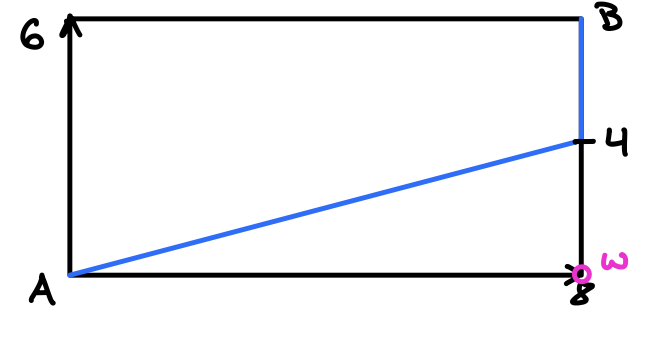
\includegraphics[width=.5\textwidth]{images/2019_20_1.png}
\end{figure}
}
\end{enumerate}
}
{
\subsubsection*{Exercise 2}

\begin{enumerate}
    \item LNS of preferences
    \item complete markets
    \item free disposal
\end{enumerate}

Suppose (1) is violated. Then we could construct the following situation (A violates LNS):

\begin{figure}[!htp]
    \centering
    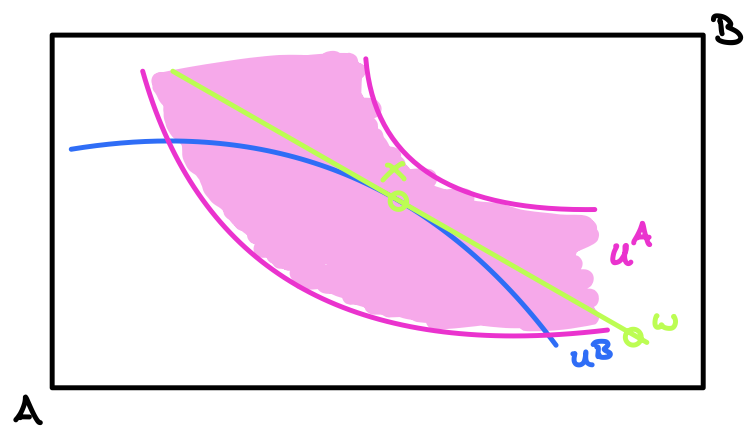
\includegraphics[width=.75\textwidth]{images/2019_20_2.png}
\end{figure}

Although at $x$ both agents are optimizing given the prices, we could make $B$ better off without hurting $A$ if we moved to the bottom left. Thus the CE at $x$ is not PE.
}
{
\subsubsection*{Exercise 3}

\begin{align*}
    \left(w_{1}, w_{2}\right)=(9,16)
\end{align*}

\begin{enumerate}[label=(\alph*)]
{\item 
$$
\begin{array}{ll}
t=0: & q_{1} \theta_{1}+q_{2} \theta_{2}=0 \\
t=1 \text { and } s=1: & x_{1}=w_{1}+\theta_{1}+3 \theta_{2}=9+\theta_{1}+3 \theta_{2} \\
t=1 \text { and } s=2: & x_{2}=w_{2}+3 \theta_{1}+\theta_{2}=16+3 \theta_{1}+\theta_{2}
\end{array}
$$
}
{\item 
Solve the maximization problem. I already substitute $x_{1}$ and $x_{2}$ from the BC s into the EU-function :

$$
\begin{gathered}
\max _{\theta_{1} \theta_{2}} \frac{1}{2}\left[\sqrt{9+\theta_{1}+3 \theta_{2}}+\sqrt{16+3 \theta_{1}+\theta_{2}}\right] \\
\text { st. } \quad q_{1} \theta_{1}+q_{2} \theta_{2}=0
\end{gathered}
$$

FOC:

$$
\begin{aligned}
& \frac{1}{2}\left[\frac{1 / 2}{\sqrt{9+\theta_{1}+3 \theta_{2}}}+\frac{1 / 2 \cdot 3}{\sqrt{16+3 \theta_{1}+\theta_{2}}}\right]-\lambda q_{1}=0 \\
& \frac{1}{2}\left[\frac{1 / 2 \cdot 3}{\sqrt{9+\theta_{1}+3 \theta_{2}}}+\frac{1 / 2}{\sqrt{16+3 \theta_{1}+\theta_{2}}}\right]-\lambda q_{2}=0
\end{aligned}
$$

Since there is only one consumer. must have no trade equilibrium: $\theta_{1}=\theta_{2}=0$. Plug into FOCs:

$$
\begin{aligned}
    \frac{1}{2}\left[\frac{1 / 2}{3}+\frac{1 / 2 \cdot 3}{4}\right]-\lambda q_{1}=0 &\Longleftrightarrow \lambda q_{1}=\frac{1}{4}\left[\frac{1}{3}+\frac{3}{4}\right]=\frac{13}{4 \cdot 12} \\
    \frac{1}{2}\left[\frac{1 / 2 \cdot 3}{3}+\frac{1 / 2}{4}\right]-\lambda q_{2}=0 &\Longleftrightarrow \lambda q_{2}=\frac{1}{4}\left[1+\frac{1}{4}\right]=\frac{5}{4 \cdot 4} \\
    \longrightarrow & \frac{q_{1}}{q_{2}}=\frac{13}{12} \cdot \frac{4}{5}=\frac{13}{15}
\end{aligned}
$$
}
{\item 
$\mathbb{E}\left(r_{1}\right)=\frac{1}{2}(1+3)=2=\mathbb{E}\left(r_{2}\right)=\frac{1}{2}(3+1)$

Thus:

$$
\frac{q_{1}}{q_{2}}<1 \Longleftrightarrow \frac{1}{q_{2}}<\frac{1}{q_{1}} \Leftrightarrow \frac{\mathbb{E}\left(r_{1}\right)}{q_{1}}>\frac{\mathbb{E}\left(r_{2}\right)}{q_{2}}
$$

The expected rate of return for asset 1 is larger than for asset 2.

Since the consumer is richer in state 2 and risk-averse, she would like to buy asset 2 as insurance. Because she is alone in the economy, this demand for asset 2 increases $q_{2}$ relative to $q_{1}$. This in turn leads to $\frac{1}{q_{1}}>\frac{1}{q_{2}}$ and $\frac{\mathbb{E}\left(r_{1}\right)}{q_{1}}>\frac{\mathbb{E}\left(r_{2}\right)}{q_{2}}$.
}
\end{enumerate}
}
}\newpage
\section{Microeconomics Midterm 2020 / 21}

{
\subsection*{Schmidt}

{
\subsubsection*{Exercise 1}

\begin{enumerate}[label=(\alph*)]
{\item 
$x_{1}\left(\lambda p_{1} \lambda w\right)=\lambda^{1+\alpha-\delta} \frac{p_{1}^{\alpha} w}{p_{1}^{\delta}+p_{2}^{\delta}+p_{3}^{\delta}}=\lambda^{1+\alpha-\delta} x_{1}(p, w)$

Must have $\alpha=\delta-1$

$$
x_{2}\left(\lambda p_{1} \lambda w\right)=\lambda^{1+\alpha-\delta} \frac{p_{2}^{\alpha} w}{p_{1}^{\delta}+p_{2}^{\delta}+p_{3}^{\delta}}+\beta \frac{p_{1}}{p_{3}} \frac{\lambda}{\lambda}
$$

No restriction on $\beta$.

$$
x_{3}(\lambda p, \lambda w)=\lambda^{1+\alpha-\sigma} \frac{\gamma p_{3}^{\alpha} w}{p_{1}^{\delta}+p_{2}^{\delta}+p_{3}^{\delta}}=\lambda^{1+\alpha-\delta} x_{3}(p, w)
$$

No restriction on $\gamma$.

In summary, we only need $\alpha=\delta-1$
}
{\item 
$p_{1} x_{1}(\cdot)+p_{2} x_{2}(\cdot)+p_{3} x_{3}(\cdot)=w$ to satisfy Walras' Law

$$
\frac{w}{p_{1}^{\delta}+p_{2}^{\delta}+p_{3}^{\delta}}\left[p_{1}^{1+\alpha}+p_{2}^{1+\alpha}+\gamma p_{3}^{1+\alpha}\right]+\beta \frac{p_{1} p_{2}}{p_{3}}=w
$$

Must have $\beta=0$ :

$$
p_{1}^{\delta}+p_{2}^{\delta}+p_{3}^{\delta}=p_{1}^{1+\alpha}+p_{2}^{1+\alpha}+\gamma p_{3}^{1+\alpha}
$$

Must have $\gamma=1$ \& $\alpha=\delta-1$.

In summary:

$$
\alpha=\delta-1 \quad \beta=0 \quad \gamma=1
$$
}
\end{enumerate}
}
{
\subsubsection*{Exercise 2}

(1) Define $\tilde{\alpha}_{1}=\frac{\alpha_{1}}{\alpha_{1}+\alpha_{2}}$ and $\tilde{\alpha}_{2}=\frac{\alpha_{2}}{\alpha_{1}+\alpha_{2}}$. Then

$$
u\left(x_{1}, x_{2}\right)=\left(x_{1}-\gamma_{1}\right)^{\tilde{\alpha}_{1}}\left(x_{2}-\gamma_{2}\right)^{\tilde{\alpha}_{2}}
$$

and $\tilde{\alpha}_{1}+\tilde{\alpha}_{2}=1$. This is allowed as it is a monotone transformation of utility.

(2) Define $\tilde{x}_{1}=\left(x_{1}-y_{1}\right)$ and $\tilde{x}_{2}=\left(x_{2}-y_{2}\right)$.

At the same time let $\tilde{w}=w-p_{1} y_{1}-p_{2} y_{2}$.

The intuition is that we only allow the consumer to choose the excess consumption after
obtaining at least $\gamma_{1}$ (or $\gamma_{2}$). For example, let $x_{1}$ be food and you need $\gamma_{1}$ food or you die. Thus you are only free to choose excess food after having $\gamma_{1}$. To make the budget work, I subtract the expenses for $\gamma_{1}$ (and $\gamma_{2}$ ) from the income.

(3) Now we get an immediate solution as the new problem is just standard Cobb-Douglas:

$$
\begin{aligned}
& \max _{\tilde{x}_{1}, \tilde{x}_{2}} \tilde{x}_{1}^{\tilde{\alpha}_{1}} \tilde{x}_{2}^{\tilde{\alpha}_{2}} \\
& \text { s.t. } p_{1} \tilde{x}_{1}+p_{2} \tilde{x}_{2}=\tilde{w} \\
& \rightarrow \tilde{x}_{1}=\tilde{\alpha}_{1} \frac{\tilde{w}}{p_{1}} \quad ; \quad \tilde{x}_{2}=\tilde{\alpha}_{2} \frac{\tilde{w}}{p_{2}}
\end{aligned}
$$

(4) Re-substitute:

$$
\begin{aligned}
& \left(x_{1}-\gamma_{1}\right)=\tilde{\alpha}_{1} \frac{1}{p_{1}}\left(w-p_{1} y_{1}-p_{2} \gamma_{2}\right) \\
& \Leftrightarrow \quad \quad p_{1} x_{1}=p_{1} \gamma_{1}+\tilde{\alpha}_{1}\left(w-p_{1} \gamma_{1}-p_{2} \gamma_{2}\right)
\end{aligned}
$$

By symmetry:

$$
p_{2} x_{2}=p_{2} \gamma_{2}+\tilde{\alpha}_{2}\left(w-p_{1} \gamma_{1}-p_{2} \gamma_{2}\right)
$$
}
{
\subsubsection*{Exercise 3}

\begin{enumerate}[label=(\alph*)]
{\item 
Cost is: $c(\cdot)=w_{1} z_{1}(\cdot)+w_{2} z_{2}(\cdot)$

Then:

\begin{align*}
    \quad \frac{\partial c(\cdot)}{\partial w_{1}}=z_{1}(\cdot)+w_{1} \frac{\partial z_{1}(\cdot)}{\partial w_{1}}+w_{2} \frac{\partial z_{2}(\cdot)}{\partial w_{1}} \tag{I}
\end{align*}

The firm solves

\begin{align*}
\max_{z_{1} z_{2}} p f\left(z_{1}, z_{2}\right)-w_{1} z_{1}-w_{2} z_{2}
\end{align*}

FOC:

\begin{align*}
& p \frac{\partial f(\cdot)}{\partial z_{1}}-w_{1}=0 \Leftrightarrow w_{1}=p \frac{\partial f(\cdot)}{\partial z_{1}}  \tag{II}\\
& p \frac{\partial f(\cdot)}{\partial z_{2}}-w_{2}=0 \Leftrightarrow w_{2}=p \frac{\partial f(\cdot)}{\partial z_{2}} \tag{III}
\end{align*}
Plug (II) and (III) into (I):

\begin{align*}
\frac{\partial c(\cdot)}{\partial w_{1}} & =z_{1}(\cdot)+p \frac{\partial f(\cdot)}{\partial z_{1}} \frac{\partial z_{1}(\cdot)}{\partial w_{1}}+p \frac{\partial f(\cdot)}{\partial z_{2}} \frac{\partial z_{2}(\cdot)}{\partial w_{2}} \\
& =z_{1}(\cdot)+p\left[\frac{\partial f(\cdot)}{\partial w_{1}}+\frac{\partial f(\cdot)}{\partial w_{2}}\right]=z_{1}(\cdot)
\end{align*}
}
{\item 
If production is below 2 units, then $c_1\left(y_{1}\right)$ is more cost efficient. Above 2 units, the firm can reduce cost by switching to $c_{2}\left(y_{2}\right)$ :

$$
c(y)= \begin{cases}y^{2} / 2 & \text { if } y<2 \\ y & \text { if } y \geqslant 2\end{cases}
$$
}
\end{enumerate}
}
{
\subsubsection*{Exercise 4}

\begin{enumerate}[label=(\alph*)]
{\item 
The agent maximizes expected utility:

$$
\max _{A} \int u\left(w-A+Az\right) d F(z)
$$

Getting the first coder derivative:

\begin{equation*}
\frac{\partial E U}{\partial A}=\int u^{\prime}(w-A+A z)(z-1) d F(z) \tag{IV}
\end{equation*}

Suppose $A=0$ :

$$
\begin{aligned}
\frac{\partial E U}{\partial A}(A=0) & =\int u^{\prime}(w)(z-1) d F(2) \\
& =u^{\prime}(w)\left[\int z d F(z)-1\right]>0
\end{aligned}
$$

As marginal expected utility is strictly positive, the agent would be marginally better off by investing $A>0$. Thus, she would always do so.
}
{\item 
CARA implies $u(x)=\exp (-r x)$ since

$$
-\frac{u^{\prime \prime}(x)}{u^{\prime}(x)}=-\frac{r^{2} \exp (-r x)}{-r \exp (-r x)}=r
$$

Go back to (IV) and set equal to zero for optimality condition:

$$
\int u^{\prime}(w-A+A z)(z-1) d F(z)=0
$$

Plug in $u^{\prime}(x)=-r \exp (-r x)$ :

\begin{align*}
& \int-r \exp (-r(w-A+A z))(z-1) d F(z)=0 \\
\Leftrightarrow & \underbrace{-r \exp (-r(w-A))}_{\neq 0} \int \exp \left(-r Az\right)(z-1) d F(z)=0 \\
\Leftrightarrow & \int \exp \left(-r Az\right)(z-1) d F(z)=0 \tag{V}
\end{align*}

(V) implicitly defines the optimal A and does not depend on wealth.
}
\end{enumerate}
}
}

{
\subsection*{Gottardi}

{
\subsubsection*{Exercise 1}

\begin{enumerate}[label=(\alph*)]
{\item 
Must have $c \leq y=2 L$ and $L=16-l$

Thus: $c \leqslant 32-2 l$ describes feasible allocations. PE allocations are only at $c=32-2 l$, as otherwise, resources are wasted that could contribute towards utility:

\begin{figure}[!htp]
    \centering
    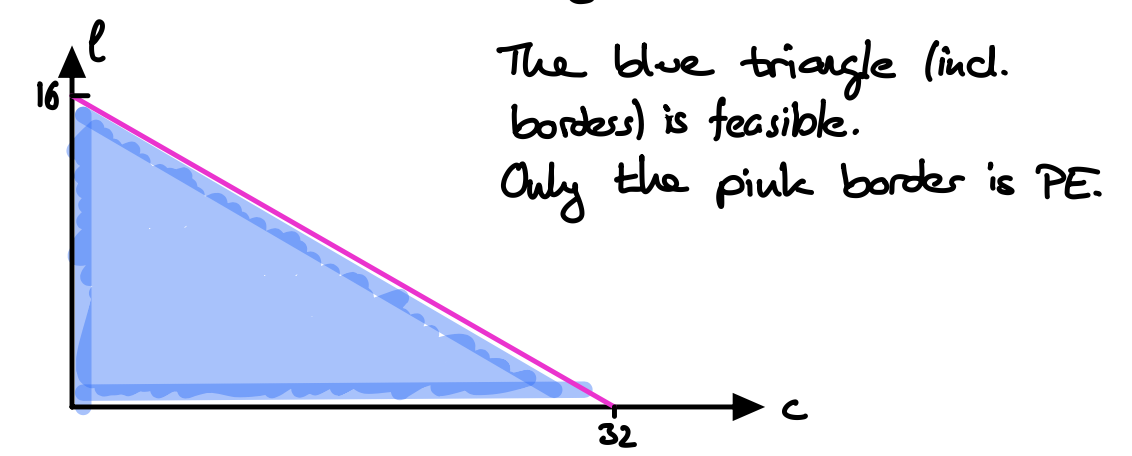
\includegraphics[width=.75\textwidth]{images/2020_21_1.png}
\end{figure}
}
{\item 
\underline{consumer:}

\begin{align*}
    \max _{c, l} \ln (c)+\ln (l) \\
    \text { st. } p c+w l=16 w
\end{align*}

FOCs:

\begin{align*}
    & \frac{1}{c}-\lambda p=0 \\
    & \frac{1}{c}-\lambda w=0 \\
    &\rightarrow c=\frac{w}{p} l
\end{align*}

\underline{Firm:}

\begin{align*}
    \max P A L-w L
\end{align*}

$$
L=\left\{\begin{array}{lll}
\infty & \text { if } & A \geq w / p \\
\mathbb{R}^{+} & \text {if } & A \geq w / p \\
0 & \text { if } & A<w / p
\end{array}\right.
$$

\underline{Markets:}

\begin{align*}
    L=16-l \longrightarrow w / p=A=2
\end{align*}

$$
\begin{aligned}
& \left\lvert\, \begin{array}{l}
c=y=A L=A(16-l)=32-2 l \\
c=\frac{w}{p}l=A l=2 l
\end{array}\right\rvert\, \\
& \longrightarrow l=8 ; L=8 ; c=y=16
\end{aligned}
$$

\underline{Competitive Equilibrium:}

\begin{align*}
    w / p=2 \\
    y=16 \\
    L=8
\end{align*}

Since $c=32-2 l$ holds, the $C E$ is $P E$.
}
{\item 
(1) $\frac{w}{p}$ will increase, as $\frac{w}{p}=A^{\prime}$. Else, we'd have $\frac{w}{p}<A^{\prime}$ and the firm would demand infinite labour. This excess demand cannot exist in a CE.

(2) $y$ must increase. More productive firm increases its output.

(3) $L$ remains the same. The firm produces more at a lower price and the consumer consumes more, working the same for a higher relative wage. She could work more and consume more but since $MRS =c / l$, this is not what happens.

The utility increases as $l=8$ as before but $c$ increases as $y$ increases.
}
\end{enumerate}
}
{
\subsubsection*{Exercise 2}
Yes. If one of the consumers has non-convex preferences, we con find prices at PE allocations that are not CE:

\begin{figure}[!htp]
    \centering
    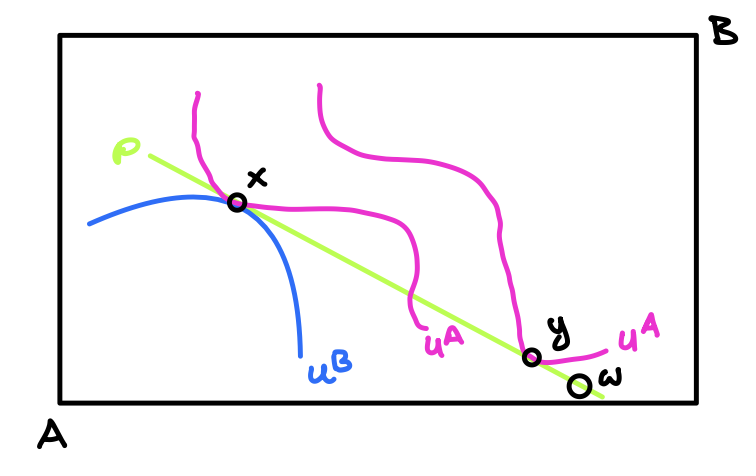
\includegraphics[width=.75\textwidth]{images/2020_21_2.png}
\end{figure}

Although $x$ is PE, A could be better off at these prices. Therefore $x$ is not a CE.
}
{
\subsubsection*{Exercise 3}

\begin{align*}
    w^{A}=(4,8) \quad ; \quad w^{B}=(2,1)
\end{align*}

\begin{enumerate}[label=(\alph*)]
{\item 
$$
MRS^{A}=\frac{1 / 2 x_{2}^{A}}{1 / 2 x_{1}^{A}} \stackrel{!}{=} M R S^{B}=1 \rightarrow x_{2}^{A}=x_{1}^{A}
$$

All PE-allocation are in blue.

\begin{figure}[!htp]
    \centering
    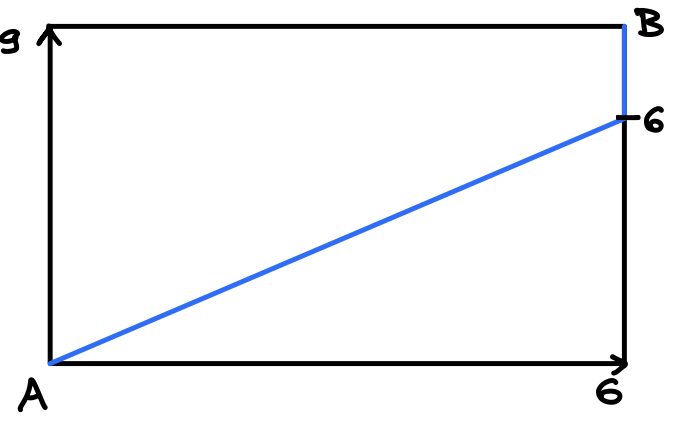
\includegraphics[width=.75\textwidth]{images/2020_21_3.png}
\end{figure}
}
{\item 
\underline{consumer A:}

\begin{align*}
    & \max_{x_{1}^{A}, x_{2}^{A}} 1 / 2\left(\ln \left(x_{1}^{A}\right)+\ln \left(x_{2}^{A}\right)\right) \\
    \text { s.t. } & q_{1} \theta_{1}^{A}+q_{2} \theta_{2}^{A}=0 \\
    & x_{1}^{A}=w_{1}^{A}+\theta_{1}^{A} \\
    & x_{2}^{A}=w_{2}^{A}+\theta_{2}^{A}
\end{align*}

\begin{align*}
    \Longleftrightarrow \quad \max _{x_{1}^{A} , x_{2}^{A}} 1 / 2\left(\ln \left(x_{1}^{A}\right)+\ln \left(x_{2}^{A}\right)\right) \\
    \text{s.t. } q_{1}\left(x_{1}^{A}-w_{1}^{A}\right)+q_{2}\left(x_{2}^{A}-w_{2}^{A}\right)=0
\end{align*}

FOCs:

\begin{align*}
    \left[x_{1}^{A}\right]: \frac{1}{2 x_{1}^{A}}-\lambda q_{1} & =0 \\
    {\left[x_{2}^{A}\right]: \frac{1}{2 x_{2}^{A}}-\lambda q_{2} } & =0 \\
    \rightarrow \frac{q_{1}}{q_{2}} &=\frac{x_{2}^{A}}{x_{1}^{A}} \tag{I}
\end{align*}

\underline{consumer B:}

\begin{align*}
    \max_{x_{1}^{\beta} x_{2}^{\beta}} 1 / 2\left(x_{1}^{\beta}+x_{2}^{\beta}\right) \\
    \text { s.t. } q_{1}\left(x_{1}^{B}-w_{1}^{D}\right)+q_{2}\left(x_{2}^{8}-w_{1}^{B}\right)=0 
\end{align*}

FOCs:


\begin{align*}
    \left[x_{1}^{B}\right]: 1 / 2+\lambda q_{1}=0 \\
    \left[x_{2}^{B}\right]: 1 / 2+\lambda q_{2}=0 \\
    \rightarrow \frac{q_{1}}{q_{2}}=1 \tag{II}
\end{align*}

Plug (II) into (I):

\begin{align*}
    x_{2}^{A}=x_{1}^{A} \tag{III}
\end{align*}

Use (II) and (III) in BC for $A$ :

$$
x_{1}^{A}=x_{2}^{A}=\frac{w_{1}^{A}+w_{2}^{A}}{2}=6
$$

\underline{markets:}

$$
\begin{aligned}
& x_{1}^{A}+x_{1}^{B}=w_{1}^{A}+w_{1}^{B}=6 \\
& \longrightarrow x_{1}^{B}=0 \\
& x_{2}^{A}+x_{2}^{B}=w_{2}^{A}+w_{2}^{B}=9 \\
& \longrightarrow x_{2}^{B}=3
\end{aligned}
$$

\underline{Competitive Equilibrium:}

$$
\begin{aligned}
\left(x_{1}^{A}, x_{2}^{A}\right) & =(6,6) \\
\left(x_{1}^{B}, x_{2}^{B}\right) & =(0,3) \\
\frac{q_{1}}{q_{2}} & =1
\end{aligned}
$$
}
{\item 

PE:

\begin{align*}
    M R S^{A}=x_{2}^{A} / x_{1}^{A} \stackrel{!}{=} M R S^{B}=1 / 3 \\
    \longrightarrow x_{2}^{A}=\frac{1}{3} x_{1}^{A}
\end{align*}

The new set of PE-allocations is indicated in pink.

\begin{figure}[!htp]
    \centering
    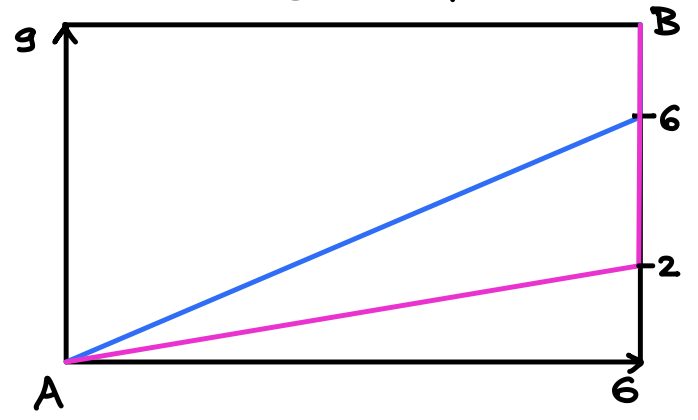
\includegraphics[width=.75\textwidth]{images/2020_21_4.png}
\end{figure}

Now $\frac{q_{1}}{q_{2}}=\frac{1}{3}$. Reason being that the prices of the Arrow-securities reflect the state-probabilities of the risk-neutral agent as she will take on the entire risk in equilibrium.
}
\end{enumerate}
}
}\newpage
\section{Microeconomics Midterm 21 / 22}

{
\subsection*{Schmidt}

{
\subsubsection*{Exercise 1}

\begin{enumerate}[label=(\alph*)]
{\item 
Clearly, WA is violated as $15 \in[0.22 .5]$ by the result in (b).
}
{\item 
WA: if $x \neq x^{\prime}$ and $p^{\prime} x \leqslant w^{\prime} \Rightarrow p x^{\prime}>w$

Thus check bundles in other price-wealth situations:

$$
\begin{aligned}
\left|\begin{array}{l}
4 \cdot 30+8 \cdot y=120+8 y \leqslant w_{0}=4 \cdot 15+8 \cdot 30=300 \\
12 \cdot 15+6 \cdot 30=360 \leqslant w_{1}=12 \cdot 30+6 y=360+6 y \\
\end{array}\right| \\
\Leftrightarrow\left|\begin{array}{l}
y \leqslant 22.5 \\
0 \leqslant y
\end{array}\right|
\Longleftrightarrow y \in[0.22 .5]
\end{aligned}
$$

$W A$ is violated if $y \in[0,22.5]$.
}
\end{enumerate}
}
{
\subsubsection*{Exercise 2}

\begin{enumerate}[label=(\alph*)]
{\item 
Use Roy's identity:

$$
x_{l}(p, w)=-\frac{\frac{\partial v(p, w)}{\partial p_{l}}}{\frac{\partial v(p, w)}{\partial w}}
$$

Then let $f(\cdot)$ be a movotonic tranformation:

$$
\tilde{x}_{l}(p, w)=-\frac{\frac{\partial f(v(p, w))}{\partial p_{l}}}{\frac{\partial f(p, w))}{\partial w}}=-\frac{\frac{\partial f(p, w)}{\partial v(p, w)}}{\frac{\partial f(p, w)}{\partial v(p, w)}} \frac{\frac{\partial v(p, w)}{\partial p_{l}}}{\frac{\partial v(p, w)}{\partial w}}=x_{l}(p, w)
$$
}
{\item 
(1) find $w(v(p, w))$ :

$$
w=\left(\frac{p_{1}}{\alpha}\right)^{\alpha}\left(\frac{p_{2}}{1-\alpha}\right)^{1-\alpha} v(p, w)
$$

At optimum: $w=e(p, u)$ and $v(p, w)=u$.

(2) Apply Shephard's Lemma to e(p,u):

$$
\begin{aligned}
h_{1}(p, u)=\frac{\partial e\left(p_{1} u\right)}{\partial p_{1}} & =\alpha\left(\frac{1}{\alpha}\right)^{\alpha}\left(\frac{p_{2}}{p_{1}(1-\alpha)}\right)^{1-\alpha} u \\
& =\left(\frac{p_{2}}{p_{1}} \frac{\alpha}{1-\alpha}\right)^{1-\alpha} u
\end{aligned}
$$
}
{\item 
case 1:

$$
\begin{aligned}
& \alpha=\alpha\left(p_1 / p_{2}\right) \longrightarrow \alpha\left(\lambda p_{1} / \lambda p_{2}\right)=\alpha \\
& h_{1}\left(\lambda p_{1}, u\right)=\left(\frac{\lambda p_{2}}{\lambda p_{1}} \frac{\alpha}{1-\alpha}\right)^{1-\alpha} u \\
& =\left(\frac{p_{2}}{p_{1}} \frac{\alpha}{1-\alpha}\right)^{1-\alpha} u=h_{1} (p_{1}, u)
\end{aligned}
$$

case 2: $\alpha=\alpha\left(p_{1}\right)$

$$
\begin{aligned}
h_{1}(\lambda p_1, u) & =\left(\frac{\lambda p_{2}}{\lambda p_{1}} \frac{\alpha\left(\lambda {p_{1}}\right)}{1-\alpha \left(\lambda p_{1}\right)}\right)^{1-\alpha\left(\lambda_{p_{1}}\right)} u \\
& =\left(\frac{p_{2}}{p_{1}} \frac{\alpha\left(\lambda p_{1}\right)}{1-\alpha\left(\lambda {p_{1}}\right)}\right)^{1-\alpha\left(\lambda_{p_{1}}\right)} u \neq h_{1}\left(p_{1} , u\right)
\end{aligned}
$$
}
\end{enumerate}
}
{
\subsubsection*{Exercise 3}

The difference between consumer theory and production theory is mainly the fact that firms do not have budget constraints.
This problem introduces a budget constraint. Therefore, we are going to treat the problem like a consumer problem.
In that sense, the revenue is comparable to the utility function, and the cash constraint is like the wealth of a consumer.
Consequently, we are solving the following revenue maximization problem (which is the analogue to a utility maximization problem):

\begin{align*}
    \max_{z_1,z_2} pf(z_1,z_2) \\
    \operatorname{s.t.} \; w_1z_1 + w_2z_2 \leq C
\end{align*}

We will assume an interior solution (the budget constraint is binding).
Then, the revenue function $R(p, w_1, w_2, C)$ that the exercise gives us is just the equivalent to the indirect utility.

\begin{enumerate}[label=(\alph*)]
{\item 
As $R(p, w_1, w_2, C)$ works like the indirect utility, we apply Roy's identity to find the factor demand, which is the analogue to the Walrasian demand:

\begin{align*}
    z_1&=-\frac{\frac{\partial R}{\partial w_1}}{\frac{\partial R}{\partial C}} \\
    &= -\frac{p \cdot(-\alpha) \frac{1}{w_1}}{p \cdot \frac{1}{C}} \\
    &= \alpha \frac{C}{w_1}
\end{align*}
}
{\item 
We treat $R(p,w,C)$ as the indirect utility depending on income and invert it to find the cost function $C(p,w,R)$, which is the analogue to the expenditure function in consumer theory:

\begin{align*}
    R&=p\left[\gamma+\ln C(p,w,R)-\alpha \ln w_1-(1-\alpha) \ln w_2\right] \\
    \frac{R}{p}-\gamma &= \ln \left(\frac{C(p,w,R)}{w_1^\alpha w_2^{1-\alpha}} \right) \\
    \exp\left(\frac{R}{p}-\gamma\right)&=\frac{C(p,w,R)}{w_1^\alpha w_2^{1-\alpha}} \\
    C(p,w,R) &= w_1^\alpha w_2^{1-\alpha}\exp\left(\frac{R}{p}-\gamma\right)
\end{align*}
}
{\item 
Since the cost function from (b) happens to be the analogue to the expenditure function, we can apply Shephard's Lemma in order to find the factor demand for a given $R$ at minimum cost, as this is the analogue to the Hicksian demand in consumer theory.
In that spirit, let us call this function $h_1(p,w,R)$.

\begin{align*}
    h_1(p,w,R)&=\frac{\partial C\left(w,R\right)}{\partial w_1} \\
    &= \alpha \exp \left[\frac{R}{p}-\gamma\right] \cdot\left(\frac{w_2}{w_1}\right)^{1-\alpha}
\end{align*}
}
{\item 
In consumer theory, the Hicksian demand and the Walrasian demand meet at optimum. We can also show that here:

\begin{align*}
    h_1(w,R)&=z_1^* \\
    \alpha \exp \left[\frac{R}{p}-\gamma\right] \cdot\left(\frac{w_2}{w_1}\right)^{1-\alpha}&=\alpha \frac{C}{w_1}\\
    \exp \left[\frac{R}{p}-\gamma\right] w_1^\alpha w_2^{1-\alpha}&=C \\
    \frac{R}{p}-\gamma &= \ln \left(\frac{C}{w_1^\alpha w_2^{1-\alpha}} \right) \\
    R&=p\left[\gamma+\ln C-\alpha \ln w_1-(1-\alpha) \ln w_2\right]
\end{align*}

The last line is exactly the formula for the revenue that is observed by our econometrician friend in the optimum. Therefore, we have shown that the two demands are equal whenever the firm is acting optimally, i.e. maximizing its revenue or minimizing its cost. Put differently, the revenue maximization problem is the dual problem to the cost minimization problem and vice versa.
}
\end{enumerate}
}
{
\subsubsection*{Exercise 4}

\begin{enumerate}[label=(\alph*)]
{\item 
\underline{IF:}

$u(x)=\beta x^{1-\rho}+\gamma$

$$
r^{R}=-x \frac{u^{\prime \prime}(x)}{u^{\prime}(x)}=-x \frac{\beta(1-  \rho)(-\rho) x^{-\rho-1}}{\beta(1-\rho) x^{-\rho}}=\rho
$$

\underline{ONLY IF:}

$r^{R}=-x \frac{u^{\prime \prime}(x)}{u^{\prime}(x)}=-x \frac{\partial \ln \left(u^{\prime}(x)\right)}{\partial x}=\rho$

$$
\begin{aligned}
& \Longleftrightarrow \quad \frac{\partial \ln \left(u^{\prime}(x)\right)}{\partial x}=-\rho \frac{1}{x} \\
& \Longleftrightarrow \int_{\underline{x}}^{x} \frac{\partial \ln \left(u^{\prime}(t)\right)}{\partial t} d t=-\rho \int_{\underline{x}}^{x} \frac{1}{t} d t \\
& \Longleftrightarrow \quad \ln \left(u^{\prime}(x)\right)-\ln \left(u^{\prime}(\underline{x})\right)=-\rho (\ln (x)-\ln (\underline{x})) \\
& \Leftrightarrow \quad u^{\prime}(x)=x^{-p} \frac{u^{\prime}(\underline{x})}{\underline{x}^{-\rho}}=x^{-\rho} \alpha \\
& \int_{\underline{x}}^{x} u^{\prime}(y) d y=\alpha \int_{\underline{x}}^{x} y^{-\rho} d y \\
& \Leftrightarrow \quad u(x)-u(\underline{x})=\frac{\alpha}{1-\rho}\left(x^{1-p}-\underline{x}^{1-p}\right) \\
& \Leftrightarrow \quad u(x)=\beta x^{1-p} + \gamma
\end{aligned}
$$

Risk aversion:

$$
\begin{aligned}
& u^{\prime \prime}(x)<0 \\
\Leftrightarrow &\beta(1-\rho)(-\rho) x^{-\rho-1}<0 \\
\Rightarrow &\beta(1-\rho) {\rho}>0
\end{aligned}
$$

This only holds when $(\beta>0$ and $\rho<1)$ or $(\beta<0$ and $\rho>1$ ).
}
\end{enumerate}
}
}

\newpage
{
\subsection*{Gottardi}

{
\subsubsection*{Exercise 1}

\begin{enumerate}[label=(\roman*)]
{\item 
Pareto Efficient:

\begin{align*}
    M R S^{A}=3 \frac{x_{2}^{A}}{x_{1}^{A}}&=M R S^{B}=\frac{1}{2} \\
    \Longleftrightarrow \quad x_{2}^{A}&=\frac{1}{6} x_{1}^{A}
\end{align*}

\begin{figure}[!htp]
    \centering
    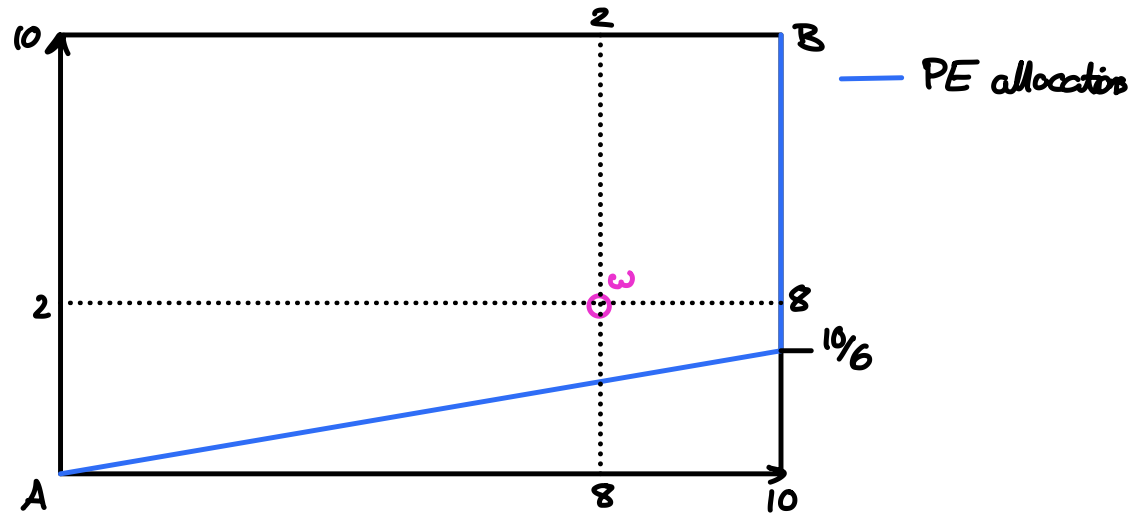
\includegraphics[width=.75\textwidth]{images/2021_22_1.png}
\end{figure}
}
{
\item 
\underline{consumer A:}

$$
\begin{aligned}
& \max _{x_{1}^{A}, x_{2}^{A}} 3 \ln \left(x_{1}^{A}\right)+\ln \left(x_{2}^{A}\right) \\
& \text { s.t. } x_{1}^{A}+p x_{2}^{A}=8+2 p 
\end{aligned}
$$

FOCs:

$$
\begin{aligned}
& \left[x_{1}^{A}\right]: \frac{3}{x_{1}^{A}}-\lambda=0 \\
& \left[x_{2}^{A}\right]: \frac{1}{x_{2}^{A}}-\lambda p=0 \\
& \rightarrow x_{1}^{A}=3 p x_{2}^{A}
\end{aligned}
$$

\underline{consumer B:} linear utility leads to:

$$
\begin{aligned}
& x_{1}^{B}=\left\{\begin{array}{lll}
\infty & \text { if } & p \geq 2 \\
\mathbb{R}^{+} & \text { if } & p=2 \\
0 & \text { if } & p<2
\end{array}\right. \\
& x_{2}^{B}=\left\{\begin{array}{lll}
\infty & \text { if } p \leq 2 \\
\mathbb{R}^{+} & \text { if } p=2 \\
0 & \text { if } p>2
\end{array}\right.
\end{aligned}
$$

\underline{market:} 

$$
x_{1}^{A}+x_{1}^{B}=10=x_{2}^{A}+x_{2}^{B}
$$

In order for markets to clear with no excess demand, we must have $p=2$ because of consumer B's preferences.
Therefore

$$
x_{1}^{A}=6 x_{2}^{A}
$$

plug into $B C^{A}: \quad 8 x_{2}^{A}=8+4 \quad \Longleftrightarrow x_{2}^{A}=12 / 8=3 / 2$

$$
\rightarrow x_{1}^{A}=9 \rightarrow\left(x_{1}^{B}, x_{2}^{B}\right)=(1,17 / 2)
$$

\underline{Competitive Equilibrium:}

\begin{align*}
    \left(x_{1}^{A}, x_{2}^{A}\right) &= (9,3 / 2) \\
    \left(x_{1}^{B}, x_{2}^{B}\right) &= (1,17 / 2) \\
    \frac{p_2}{p_1} &= 2
\end{align*}

Since $x_{2}^{A}=1 / 6 x_{1}^{A}$, PE is achieved.
}
{
\item 

$$
\begin{aligned}
& u^{A}\left(w_{1}^{A}, w_{2}^{A}\right)=3 \ln (8)+\ln (2) \cong 6.931 \\
& u^{A}\left(x_{1}^{A}, x_{2}^{A}\right)=3 \ln (9)+\ln (3 / 2) \cong 6.997 \\
& u^{B}\left(w_{1}^{B}, w_{2}^{B}\right)=2+2 \cdot 8=18 \\
& u^{B}\left(x_{1}^{D}, x_{2}^{B}\right)=1+2 \cdot 17 / 2=18
\end{aligned}
$$

By FWT this is always true, when preferences do not violate LNS, there is free disposal and markets are complete.
}
\end{enumerate}
}
{
\subsubsection*{Exercise 2}

Autarky: A sells, B buys good 1.

Effect depends on price change \& preferences.

Assume $\frac{P_1}{P_2}$ goes up (the other way round the argument can be reversed).
This makes the seller better off as she gets more per unit sold and might even sell more. For $B$ it depends on her preferences. If she can substitute and switch to selling good 1, she profits. 
If she has to buy good 1 at a higher price, she loses. It is also possible that her utility does not change despite the price change. 

If prices remain the same, nothing changes.
}
{
\subsubsection*{Exercise 3}

$$
\left(w_{1}, w_{2}\right)=(1,4)
$$

\begin{enumerate}[label=(\roman*)]
{\item 
at $t=0: \quad q_{1} \theta_{1}+q_{2} \theta_{2}=0$

at $t=1, s=1: \quad x_{1}=w_{1}+\theta_{1} 4+\theta_{2}$

at $t=1, s=2: \quad x_{2}=w_{2}+\theta_{2}$
}
{
\item 

\underline{Consumer problem:}

$$
\begin{gathered}
\max _{\theta_{1}, \theta_{2}} 1 / 4\left(w_{1}+4 \theta_{1}+\theta_{2}\right)^{1 / 2}+3 / 4\left(w_{2}+\theta_{2}\right)^{1 / 2} \\
\text { s.t. } \quad q_{1} \theta_{1}+q_{2} \theta_{2}=0
\end{gathered}
$$

FOCs:

\begin{align*}
    &\left[\theta_{1} \right]: \frac{4}{8\left(w_{1}+4 \theta_{1}+\theta_{2}\right)^{1 / 2}}-\lambda q_{1}=0 \\
    &\left[\theta_{1} \right]: \frac{1}{8\left(w_{1}+4 \theta_{1}+\theta_{2}\right)^{1 / 2}}+\frac{3}{8\left(w_{2}+\theta_{2}\right)^{1 / 2}}-\lambda q_{2}=0
\end{align*}

\underline{market clearing:}

\begin{align*}
    \theta_{1}=-\theta_{2}=0 \tag{I}
\end{align*}

Plug (I) into FOCs:

$$
\begin{aligned}
& \frac{1}{2}=\lambda q_{1} ; \quad \frac{1}{8}+\frac{3}{16}=\lambda q_{2} \\
\longrightarrow & \frac{q_{1}}{q_{2}}=\frac{1}{2} \frac{16}{5}=\frac{8}{5}
\end{aligned}
$$
}
{
\item 

$\mathbb{E}\left(r_{1}\right)=\mathbb{E}\left(r_{2}\right)=1$

$$
\longrightarrow \frac{\mathbb{E}\left(r_{1}\right)}{q_{1}}>\frac{\mathbb{E}\left(r_{2}\right)}{q_{2}} \Longleftrightarrow 1>\frac{q_{1}}{q_{2}}=\frac{8}{5}
$$

We see that the inequality above is INCORRECT, we have run into a CONTRADICTION.

Usual intuition: $q_{1} / q_{2}>1$ because consumer wants to insure against poor state where she has less income. This leads to a lower expected rate of return for asset 1. Otherwise the consumer would buy asset 1 but she cannot because of market clearing.
}
\end{enumerate}
}
}\newpage
\input{Midterms_Years/2022_23}\newpage
\input{Midterms_Years/2023_24}\newpage

\end{document}
